\documentclass[usenatbib]{latex/mn2e} 
%External Packages and personalized macros
%=========================================================================
%		EXTERNAL PACKAGES
%=========================================================================
\usepackage{amsmath} 
\usepackage{amssymb} 
\usepackage {graphicx}
%\usepackage{graphics}
\usepackage[dvips]{epsfig}
\usepackage{epsfig}  
\usepackage{color}
\usepackage[normalem]{ulem}
\usepackage{hyperref}
\usepackage{caption}

%=========================================================================
%		INTERNAL MACROS
%=========================================================================
\def\be{\begin{equation}}
\def\ee{\end{equation}}
\def\ba{\begin{eqnarray}}
\def\ea{\end{eqnarray}}

% To highlight comments 
\definecolor{red}{rgb}{1,0.0,0.0}
\newcommand{\red}{\color{red}}
\definecolor{darkgreen}{rgb}{0.0,0.5,0.0}
\newcommand{\SRK}[1]{\textcolor{darkgreen}{\bf SRK: \textit{#1}}}
\newcommand{\SRKED}[1]{\textcolor{darkgreen}{\bf #1}}

\newcommand{\LCDM}{$\Lambda$CDM~}
\newcommand{\beq}{\begin{eqnarray}}  
\newcommand{\eeq}{\end{eqnarray}}  
\newcommand{\zz}{$z\sim 3$} 
\newcommand{\apj}{ApJ}  
\newcommand{\apjs}{ApJS}  
\newcommand{\apjl}{ApJL}  
\newcommand{\aj}{AJ}  
\newcommand{\mnras}{MNRAS}  
\newcommand{\mnrassub}{MNRAS accepted}  
\newcommand{\aap}{A\&A}  
\newcommand{\aaps}{A\&AS}  
\newcommand{\araa}{ARA\&A}  
\newcommand{\nat}{Nature}  
\newcommand{\physrep}{PhR}
\newcommand{\pasp}{PASP}    
\newcommand{\pasj}{PASJ}    
\newcommand{\avg}[1]{\langle{#1}\rangle}  
\newcommand{\ly}{{\ifmmode{{\rm Ly}\alpha}\else{Ly$\alpha$}\fi}}
\newcommand{\hMpc}{{\ifmmode{h^{-1}{\rm Mpc}}\else{$h^{-1}$Mpc }\fi}}  
\newcommand{\hGpc}{{\ifmmode{h^{-1}{\rm Gpc}}\else{$h^{-1}$Gpc }\fi}}  
\newcommand{\hmpc}{{\ifmmode{h^{-1}{\rm Mpc}}\else{$h^{-1}$Mpc }\fi}}  
\newcommand{\hkpc}{{\ifmmode{h^{-1}{\rm kpc}}\else{$h^{-1}$kpc }\fi}}  
\newcommand{\hMsun}{{\ifmmode{h^{-1}{\rm {M_{\odot}}}}\else{$h^{-1}{\rm{M_{\odot}}}$}\fi}}  
\newcommand{\hmsun}{{\ifmmode{h^{-1}{\rm {M_{\odot}}}}\else{$h^{-1}{\rm{M_{\odot}}}$}\fi}}  
\newcommand{\Msun}{{\ifmmode{{\rm {M_{\odot}}}}\else{${\rm{M_{\odot}}}$}\fi}}  
\newcommand{\msun}{{\ifmmode{{\rm {M_{\odot}}}}\else{${\rm{M_{\odot}}}$}\fi}}  
\newcommand{\lya}{{Lyman$\alpha$~}}
\newcommand{\clara}{{\texttt{CLARA}}~}
\newcommand{\rand}{{\ifmmode{{\mathcal{R}}}\else{${\mathcal{R}}$ }\fi}}  

%MY COMMANDS #############################################################
\newcommand{\sub}[1]{\mbox{\scriptsize{#1}}}
\newcommand{\dtot}[2]{ \frac{ d #1 }{d #2} }
\newcommand{\dpar}[2]{ \frac{ \partial #1 }{\partial #2} }
\newcommand{\pr}[1]{ \left( #1 \right) }
\newcommand{\corc}[1]{ \left[ #1 \right] }
\newcommand{\lla}[1]{ \left\{ #1 \right\} }
\newcommand{\bds}[1]{\boldsymbol{ #1 }}
\newcommand{\oiint}{\displaystyle\bigcirc\!\!\!\!\!\!\!\!\int\!\!\!\!\!\int}
\newcommand{\mathsize}[2]{\mbox{\fontsize{#1}{#1}\selectfont $#2$}}
\newcommand{\eq}[2]{\begin{equation} \label{eq:#1} #2 \end{equation}}
%#########################################################################

\begin{document}

%=========================================================================
%		FRONT MATTER
%=========================================================================
\title{The place of the local group in the cosmic web}
\author[S. Bustamante and J.E. Forero-Romero]{
\parbox[t]{\textwidth}{\raggedright 
  Sebastian Bustamante \thanks{sbustama@pegasus.udea.edu.co}$^{1}$ 
  Jaime E. Forero-Romero$^{2}$ 
}
\vspace*{6pt}\\
$^1$Instituto de F\'{\i}sica - FCEN, Universidad de Antioquia, Calle
67 No. 53-108, Medell\'{\i}n, Colombia\\ 
$^2$Departamento de F\'{i}sica, Universidad de los Andes, Cra. 1
No. 18A-10, Edificio Ip, Bogot\'a, Colombia
}

\maketitle

\begin{abstract}


We present here a study about the influence of the environment on the
local group (LG) of galaxies in the context of $\Lambda$CDM. In this study 
we use a large volume high resolution N-body cosmological simulation 
(Bolshoi) along with the most recent methods to quantify the cosmic web 
(T-web, V-web schemes); furthermore we propose a novel approximation, base
upon the minimization of the mean density of void regions, to determinate 
the optimal threshold value $\lambda_{th}$, which have been treated until 
now as a free parameter. 
Following the recent work of Courtois et al. (2013), where was 
found that the LG is located near to a large void, we also perform an 
extensive study of voids, applying a FOF algorithm to find void regions 
and performing an analysis of their shape based upon the reduced inertia 
tensor.
Using the recent observations that constrain the tangential velocity of
M31 with respect to the Milky Way (MW), the previously established radial 
velocity, the estimated masses of dark halos, along with some criteria
to guarantee the gravitational isolation of these systems (Forero-Romero
et al. 2013-1), we select a set of halo pairs as a candidate sample 
of LG-like systems in the Bolshoi simulation. 
We look for possible biases and correlations between the environment 
properties of each LG-like system and its kinematic and formation 
properties. Among our main result we find \SRKED{[summarize our results 
here!]}.

\end{abstract}

\begin{keywords}
Cosmology: large-scale Structure of Universe, 
galaxies: star formation - line: formation
\end{keywords}


%=========================================================================
%		PAPER CONTENT
%=========================================================================

%*************************************************************************
\section{Introduction}
\label{sec:introduction}
%*************************************************************************


The spatial distribution of galaxies describes a web-like pattern, the 
so-called cosmic web. Today it is understood that such configuration is 
driven by gravitational instabilities. ...



The study of the influence of the cosmic web on galaxy properties start 
with the seminal work of Dressler \SRKED{[reference here]} and extends to 
recent works using large observational surveys that look for signatures of 
the web into the evolution of galaxy populations. With the advention of 
more detailed observations and sophisticated computational models it is 
now within our reach to understand what physical processes dominate.



This makes  that the mass assembly history of a galaxy is deeply connected 
with its  position in the cosmic web. There is an extensive body of 
literature on the effects of the web environment on the observable 
properties of galaxies. 



This environmental study is also of paramount importance to understand the 
formation of our Galaxy. In our local neighborhood, the observations of 
dwarf galaxies around the Milky Way (MW) and the Andromeda galaxy (M31) 
show filamentary and disk-like patterns that can be linked to a 
preferential infall direction, very likely connected with the cosmic web 
where the Local Group (LG) of galaxies is embedded. 



In this paper we quantify the velocity shear environment of DM halo pairs
representative of the principal members of the Local Group (LG), the Milky
Way (MW) and Andromeda galaxy (M31). We perform this study in an 
unconstrained cosmological simulation from random phases in the initial 
conditions, and unlike previous works, where were used constrained 
cosmological simulations which have been setup as to reproduce the large 
scale structure of the local universe, we use directly observational 
measurements of the kinematics properties of the local group \SRKED{
[Reference here]} in order to build faithful samples of LG-like systems.



We pay special attention to the correlation of the present velocity shear 
environment with the assembly and the kinematics properties of the pairs. 
The motivation to have that focus is that it has been previously shown 
that the LG present in three different realizations of the constrained 
simulations have assembly histories biased towards early formation times 
and absence of major mergers (ratio 1:10) in the last $10$ Gyr. In the 
case of the kinematic properties, recent observational constrains to the 
galactocentric tangential velocity of M31 has enabled to establish how 
typical is the LG in a cosmological context \SRKED{[reference to 
Forero-Romero et.al 2013-1]}, that is why we focus here how a specific kind 
of host environment biases these kinematics properties.



%*************************************************************************
\section{The Simulation}
\label{sec:the_simulation}
%*************************************************************************


As it was previously mentioned, we use an unconstrained cosmological 
simulation, the Bolshoi simulation, to identify the possible large scale 
environment of the Local Group. This is a similar approach to the one already 
used by \SRKED{[reference here]}.



The Bolshoi simulation follows the non-linear evolution of a dark matter 
density field on a cubic volume of size $250$\hMpc sampled with $2048^3$ 
particles. The cosmological parameters in the simulation are 
$\Omega_{\rm m}=0.27$, $\Omega_{\Lambda}=0.73$, $h=0.70$, $n=0.95$ and 
$\sigma_{8}=0.82$ for the matter density, cosmological constant, 
dimensionless Hubble parameter, spectral index of primordial density 
perturbations and normalization for the power spectrum. The mass of each 
particle in the simulation is $m_{\rm p}=1.4\times 10^{8}$\hMsun.



%-------------------------------------------------------------------------
\subsection{Halos and Merger Trees}
\label{subsec:halos_merger_trees}
%-------------------------------------------------------------------------



We identify halos with two algorithms, the Friends-of-Friends \SRKED{
[reference here]} algorithm and the Bound Density Maximum algorithm. The 
constructed catalogues also provide the basis for the mass aggregation 
history studies. We also include in the catalogues information about the 
substructure.



All the results presented here must be interpreted in term of host halos, 
without any information of the substructure. In particular the merger of 
two FOF halos corresponds to the epoch of first overlap, and not to the 
fusion and/or disruption of an accreted sub-halo with a dominant halo. 



The linking length is $b=0.17$ times the mean inter-particle separation. 
All objects with 20 particles or more are considered a bona fide halo and 
are included in the construction of the merger tree, this corresponds to a 
minimum halo mass of $M_{\rm min}=2.70\times 10^{9}$\hMsun in the Bolshoi 
simulation.



The halo identification for the simulation was done for XX snapshots in 
the redshift range $0<z<7$ more or less evenly spaced in look-back time.



%*************************************************************************
\section{Algorithms to quantify the cosmic web}
\label{sec:algorithms_cosmic_web}
%*************************************************************************



%-------------------------------------------------------------------------
\subsection{The tidal web (T-web)}
\label{subsec:Tweb}
%-------------------------------------------------------------------------



The first algorithm  we use to identify the cosmic web is based upon the
diagonalization of the tidal tensor, defined as the Hessian of a 
normalized gravitational potential  


%.........................................................................
%Tidal Tensor
\begin{equation}
T_{\alpha\beta} = \frac{\partial^2\phi}{\partial x_{\alpha}\partial x_{\beta}}
\end{equation}
%.........................................................................
where the physical gravitational potential has been rescaled by a factor 
$4\pi G\bar{\rho}$ in such a way that $\phi$ satisfies the following 
equation



%.........................................................................
%Poisson
\begin{equation}
\nabla^2\phi = \delta,
\end{equation}
%.........................................................................
where $\bar{\rho}$ is the average density in the Universe, $G$ is the 
gravitational constant and $\delta$ is the dimensionless matter 
overdensity.



%-------------------------------------------------------------------------
\subsection{The velocity  web (V-web)}
\label{subsec:Vweb}
%-------------------------------------------------------------------------



We also use a kinematical method to define the cosmic-web environment in 
the simulation. The method has been thoroughly described in XXX and 
applied to study the shape and spin alignment in the Bolshoi simulation 
here XX. We refer the reader to these papers to find a detailed 
description of the algorithm, its limitations and capabilities. Here we 
summarize the most relevant points for the discussion. 



The V-web method for environment finding is based on the local shear 
tensor calculated from the smoothed DM velocity field in the simulation.
The central quantity is the following dimensionless quantity 


%.........................................................................
%V-Web Definition
\eq{V_web}
{
\Sigma_{\alpha\beta} = -\frac{1}{2H_0}\pr{\frac{\partial v_{\alpha}}
{\partial x_{\beta}}+\frac{\partial v_{\beta}}{\partial x_{\alpha}}}
}
%.........................................................................
where $v_{\alpha}$ and $x_{\alpha}$ represent the $\alpha$ component of 
the comoving velocity and position, respectively. $\Sigma_{\alpha\beta}$ 
can be represented by a $3\times 3$ symmetric matrix with real values,
that ensures that is possible to diagonalize and obtain three real 
eigenvalues $\lambda_{1} > \lambda_{2}>\lambda_3$ whose sum (the trace of
$\Sigma_{\alpha\beta}$) is proportional to the divergence of the local 
velocity field smoothed on the physical scale ${\mathcal R}$. 



The relative strength of the three eigenvalues with respect to a threshold
value $\lambda_{th}$ allows for the local classification of the matter 
distribution into four web types: voids, sheets, filaments and peaks, 
which correspond to regions with 3, 2, 1 or 0 eigenvalues with values 
larger than $\lambda_{th}$. Below we shall discuss a novel approach to 
define an adequate threshold value based on the visual impression of void
regions, furthermore we study other possible values based on other visual
features of the cosmic web.



%-------------------------------------------------------------------------
\subsection{The cosmic web in Bolshoi}
\label{subsec:web_in_simulations}
%-------------------------------------------------------------------------



Both established schemes to quantify the cosmic web depend on continuous 
and smooth physical quantities, as the peculiar velocity field and the 
density field. In order to calculate the necessary tensors, a discretization
of the simulation volume is performed, so all the properties are reduced 
to single values associated to discrete cells. According to this, we divide 
the overall volume into $(256)^3$ cells, so each cell has an associated 
comoving cubic volume of $0.98 \mbox{ Mpc h}^{-1}$. Finally, in order to 
reduce possible effects due to the discretization process, a gaussian 
softening is performed between neighbour cells.



Once defined the numerical details about the classification schemes, we 
shall analyse the dependence on the threshold value $\lambda_{th}$ for each 
one. In Figure \ref{fig:mean_density} we show the variation of the mean 
density parameter $\delta$ with the threshold value for cells marked as one 
of the two more dominant types of environment (voids and sheets).



As was previously established by \SRKED{Hoffman et al. (2012)} and as 
can be seen in Figure \ref{fig:mean_density}, the behaviour of the 
V-web scheme is significantly more sensible to variations of the 
$\lambda_{th}$ value compared with the T-web scheme; nevertheless, the 
behaviour of the mean density parameter for voids, sheets and filaments, 
are qualitatively quite similar for the two schemes, increasing with the 
value of $\lambda_{th}$. Although we shall focus our analysis on voids 
because they are completely dominant in the visual impression of the 
cosmic web, an analogous analysis might be performed for other type of 
environments.



On cosmic scales, the presence of highly non-linear structures implies the 
existence of very vast regions with density lower than the mean 
cosmological value due to the mass conservation. That is why the visual 
impression of the cosmic web must be necessarily dominated by these 
under-dense regions. Keeping that in mind, our novel proposal is based upon
the correct quantification of these regions, so the optimal threshold 
value must be chosen such that: sheet regions do not invade real void 
regions (in such case, the mean density parameter of sheet regions would 
become negative) and void regions do not invade real sheet and filament 
regions (in such case, the mean density parameter of void regions would 
increase due to the contribution of over-dense regions). Thus, the optimal 
value is simply where the mean density parameter of sheet regions is 
null. According to this, we obtain the next optimal threshold values 
for the T-web and the V-web respectively, $\lambda_{opt}^T = 0.326$ and 
$\lambda_{opt}^V = 0.188$. To verify our analysis, we show in Figure 
\ref{fig:visual_impression} the visual impression for each defined critical 
value, and as can be seen, the chosen values reproduce properly the 
expected impression according to the density field. 



Our classification scheme may be thought as a refinement of the recent 
schemes, where the threshold value is used to taking as a free parameter, 
based on the classic methods, where the classification is performed 
based on a cut off of the density field directly \SRKED{[references here]}.
So we make use of the objectivity achieved by the analysis of the mean 
density, but keeping all the environmental information provided by the
tensorial schemes instead of the poor description provided by the density 
field.



%-------------------------------------------------------------------------
\subsection{Method to find void regions}
\label{subsec:method_voids}
%-------------------------------------------------------------------------



Following the recent work of \SRKED{Courtois et al. 2013}, we use a method 
based on a FOF-like algorithm to find extended regions of voids in order 
to select halo systems according to the proximity to those regions. 
To achieve this, we build the input catalogue of the FOF method with the 
positions of the center coordinate of every cell marked as void according 
to the web scheme adopted; furthermore we set an adequate linking length 
to connect even diagonal neighbour cells.



Following the work of \SRKED{Forero-Romero et al. 2008}, we also perform a 
percolation analysis in order to select the best threshold parameter that
reduce percolation in cells, thereby accounting for physical void regions.
In Figure \ref{fig:percolation_analysis} we show the obtained result 
of our percolation analysis for both web schemes. In both cases it can be 
noted the volume of the largest void region is minimized and the volume 
distribution of voids is relatively flat at $\lambda_{th} = 0.0$, that 
means percolation is completely reduced for this threshold value. So 
despite of the previously established $\lambda_{th}$ optimal values for 
each scheme, we shall use $\lambda_{th} = 0.0$ just for the detection of 
void regions. Besides, due to the domination of the large scale visual 
impression by voids, it is inevitable the presence of percolation 
phenomenon, so the current chosen threshold value for percolation is 
justified because in spite of voids are necessarily connected, we are just 
interested in detecting bulk regions.



Next, we shall calculate the reduced inertia tensor of each void region 
in order to determinate their principal directions of inertia and analyse 
the size-shape distribution of voids.


%.........................................................................
%Reduced inertia tensor
\eq{ReducedIntertia}
{ \tau_{ij} = \sum_l \frac{ x_{l,i}x_{l,j}  }{R_l^2} }
%.........................................................................
where $l$ is a index associated to each cell of to the current region, 
$i$ and $j$ indexes run over each spatial direction and finally 
$R_l$ is defined as $R_l^2 = x_{l,1}^2 + x_{l,2}^2 + x_{l,3}^2$, all 
positions are measured from the respective center of mass of the region.



The eigenvalues of the reduced inertia tensor, i.e. the principal moments
of inertia, are used to quantify the shape of void regions. They are 
denoted as $\tau_1$, $\tau_2$ and $\tau_3$ such that $\tau_1 \leq \tau_2
\leq \tau_3$. In Figure \ref{fig:distro_inertia} we show the computed
distributions for $\tau_1/\tau_2$ and $\tau_2/\tau_3$, where we rather 
calculate histograms for these ratio quantities instead of each value in 
order to avoid using an arbitrary normalization. For both schemes, it can 
be noticed that the shape-distribution is completely spread out, thereby 
indicating a non-preferred geometry of void regions, which is in agreement 
with the well-established anisotropic flow of matter associated to this 
type of region \SRKED{[reference here]}. Because of that, we shall look 
for possible alignments between the plane of rotation of halo pairs and
the principal directions of inertia of the nearest void regions.



%*************************************************************************
\section{Defining Samples}
\label{section:Def_Samples}
%*************************************************************************



In order to establish an adequate set of criteria to define a LG-like 
sample in unconstrained simulations, we proceed from the the general dark 
halo catalogues, constructed using the FOF scheme with a linking length of 
$b=0.17$ and the Bound Density Maxima (BDM) scheme for halos with an 
associated overdensity value of $200$ times the critical density 
(\SRKED{[references here]}). These samples are defined over all the Bolshoi 
simulation and will be referred as General Halos samples, \GHFOF and 
\GHBDM respectively\footnote{For each sample defined, there will be a FOF 
sample and a BDM sample in order to have robust results}. To be consistent 
with the mass range observationally determined of halos that host disk-form 
galaxies, we select halos in the mass range $7\times10^{11} < M_{h}/\hMsun 
< 7\times 10^{12}$, referred here as Individual Halos (\texttt{IH}) samples. 



As a primal approach to define gravitational bounded halo pairs we select 
halos within the \texttt{IH} sample that satisfied to be the closest to 
each other. They constitute the Pairs (\texttt{P}) sample. To maintain the 
consistency with previous works regarding algorithms used for LG selection 
(\SRKED{[references here]}), we define here the next list of conditions 
that have to fulfil a pair system in order to belong to the Isolated Pairs 
(\texttt{IP}) sample. All these considerations are based upon the relative 
dynamics of the Milky Way and M31, and its isolation from massive 
structures:



%.........................................................................
%Isolated pairs criteria
\begin{enumerate}

\item{With respect to each halo, there cannot be any other halo within the 
mass range $7\times10^{11} < M_{h}/\hMsun < 7\times 10^{12}$ closer than 
its partner. It means that there cannot be ambiguity on the identity of
the pair members.}

\item{The relative radial velocity between the two halos must be 
negative.}

\item{The distance between the center of the two halos must be less than 
$1.0$\hMpc.}

\item{The distance to any halo more massive than any of the pair members 
cannot be less than $3$\hMpc.}

\item{The distance to cluster-like halos with masses larger than 
$7\times10^{13}$ \hMsun must be larger than $4$\hMpc.}
\end{enumerate}
%.........................................................................



Following the previous criteria established by Forero-Romero et al. 2013-1,
we define a more reduced sample, the Reduced Isolated Pairs sample 
(\texttt{RIP}), as pairs that fulfil the next two extra criteria :



%.........................................................................
%Reduced Isolated pairs criteria
\begin{enumerate}

\item{The separation between the center of mass of the halos is in the 
range $700-800$kpc.}

\item{The total mass of the two halos is in the range 
$1-4\times 10^{12}/\hMsun$.}

\end{enumerate}
%.........................................................................



Finally in Table \ref{tab:Samples_Size} shows the sizes of all defined 
samples. 


%.........................................................................
%Table of sizes of each sample defined in Bolshoi
\begin{table}[h]
\begin{flushleft}
\begin{center}
  \begin{tabular}{l  r  r} \hline\hline
	\textbf{Sample}					&\textbf{FOF}&\textbf{BDM} \\ \hline
	General Halos (\texttt{GH}) 	& 432000	 & 404432  \\ 
	Individual Halos (\texttt{IH}) 	& 65109		 & 61165  \\ 
	Pairs (\texttt{P}) 	 			& 17115		 & 15981  \\ 
	Isolated Pairs (\texttt{IP})	& 1249		 & 1647  \\ 
	Reduced Isolated Pairs (\texttt{RIP})& 138	 & 116  \\ \hline\hline
  \end{tabular}  
  \captionof{table}{\small Size of each sample defined in the Bolshoi 
  simulation and for each of the two schemes used to detect halos (FOF 
  and BDM).}
  
  \label{tab:Samples_Size}
  
\end{center}
\end{flushleft}
\end{table}
%.........................................................................


It can also be noticed that both schemes used to detect halos in the 
simulation are practically equivalent regarding the size of each sample.


%*************************************************************************
\section{Finding the Environment of the Local Group}
\label{sec:LGEnvironment}
%*************************************************************************



Once defined all samples, we shall proceed to quantify the environment
by using two different approaches. The first one is by applying the 
tensorial schemes defined in Section \ref{sec:algorithms_cosmic_web} 
and then, calculating the local eigenvalues associated to each halo or halo 
pair and the respective fractional anisotropy index (\SRKED{[reference 
here]}). The second approach is complementary to the first one, and 
consists in calculating the relative distance of each halo or halo pair to 
the nearest void regions, thereby allowing linking the influence of bulk 
voids to physical properties of the samples.




%-------------------------------------------------------------------------
\subsection{Tensorial Schemes}
\label{subsec:tensorial_schemes}
%-------------------------------------------------------------------------



The advantage of using the tensorial schemes (T-web and V-web) defined in
Section \ref{sec:algorithms_cosmic_web}, lies in quantifying all the local 
structure of the environment of halos and pair halos just from kinematic 
and dynamic properties of the matter distribution, like the density and 
velocity fields. Next, we shall calculate the distributions of each 
eigenvalue for the two defined web schemes and for the \texttt{GH}, 
\texttt{IP} and \texttt{RIP} samples. In Figure \ref{fig:distro_cosmicweb} 
is shown the obtained results, where it can be noticed that there is a 
significant bias in the distribution of halo pairs respect to volume cells. 
Furthermore, choosing the previously established optimal threshold value 
$\lambda_{opt}$ for each web scheme, Table \ref{tab:OccupationFractions} 
is built. In this has been listed the occupation fractions for the volume 
cells of the simulation and for each sample defined in the previous Section 
\ref{section:Def_Samples}.



%.........................................................................
%Table of 
\begin{table}[H]
\begin{flushleft}
\begin{center}
  \begin{tabular}{l  r  r  r  r}
  	&&\textbf{T-web}&&\\\hline\hline
	\textbf{Region}	&\textbf{void}&\textbf{sheet}&\textbf{filament}&\textbf{knot}	\\\hline
	Cells			&	60.6\%	  &		29.1\%	 &		9.7\%	   &	0.7\%		\\
	&&&&\\	
	\GHFOF			& 	12.1\%	  &		35.9\%	 &		43.3\%	   &	8.7\%		\\
	\GHBDM			&	9.7\%	  &		31.9\%	 &		44.2\%	   &	14.2\%		\\
	&&&&\\	
	\IPFOF			&	0.1\%	  &		6.1\%	 &		63.3\%	   &	30.5\%		\\
	\IPBDM			&	0.1\%	  &		3.0\%	 &		53.3\%	   &	43.6\%		\\
	&&&&\\
	\RIPFOF			&	0.0\%	  &		5.1\%	 &		88.4\%	   &	6.5\%		\\
	\RIPBDM			&	0.0\%	  &		3.4\%	 &		85.3\%	   &	11.2\%		\\\hline\hline
	&&&&\\
  	&&\textbf{V-web}&&\\\hline\hline
	\textbf{Region}	&\textbf{void}&\textbf{sheet}&\textbf{filament}&\textbf{knot}	\\\hline
	Cells			&	49.3\%	  &		38.3\%	 &		11.3\%	   &	1.1\%		\\
	&&&&\\
	\GHFOF			&	22.7\%	  &		44.3\%	 &		29.3\%	   &	3.7\%		\\
	\GHBDM			&	20.7\%	  &		43.6\%	 &		31.6\%	   &	4.2\%		\\
	&&&&\\
	\IPFOF			&	13.3\%	  &		63.6\%	 &		23.1\%	   &	0.1\%		\\
	\IPBDM			&	10.7\%	  &		60.1\%	 &		28.4\%	   &	0.8\%		\\
	&&&&\\
	\RIPFOF			&	20.3\%	  &		68.1\%	 &		11.6\%	   &	0.0\%		\\
	\RIPBDM			&	13.8\%	  &		69.0\%	 &		17.2\%	   &	0.0\%		\\\hline\hline
  \end{tabular}  
  \captionof{table}{\small Occupation fractions for each one of the defined
  samples and for all the volume cells of the simulation, and for each one 
  of the occupied type of environment selected by both web schemes.}
  
  \label{tab:OccupationFractions}
  
\end{center}
\end{flushleft}
\end{table}
%.........................................................................



As it was mentioned, the selection of an optimal threshold value for each 
web scheme, according to our proposed method based upon the mean density, 
is just an approximation which reproduces properly the visual impression 
of the cosmic web, so Table \ref{tab:OccupationFractions} must not be 
interpreted rigorously. Those occupation values must be thought just as a 
comparative illustration in order to understand possible bias between the 
defined samples and the overall matter distribution of the simulation. For 
instance, for the T-web scheme, the occupation fraction associated to the 
\texttt{RIP} sample is greater in filaments than sheet regions, what 
should not be interpreted as \texttt{RIP} systems lie in filaments, but 
those systems lie preferentially in higher density and stronger non-linear 
regions.



An expected result obtained from Figure \ref{fig:distro_cosmicweb} is 
the equivalence between both halos detection schemes, regarding the 
obtained distribution of eigenvalues for all samples, and even for both 
web schemes. This along with the results shown in Table 
\ref{tab:Samples_Size} allow to conclude that both halos detection schemes 
reproduce reliable halos samples with similar spatial distribution since 
the occupation values of each sample are approximately equal. Regarding 
the differences between both web classification schemes, from the 
distribution of the web eigenvalues associated to volume cells, shown in 
Figure \ref{fig:distro_cosmicweb}, it is clear that each scheme quantify 
the structure of the cosmic web in very different ways, what can be 
explained by how each scheme is built. The T-web is built based upon the 
gravitational potential, thereby retaining bulk features of the cosmic web 
because of the long-range nature of the potential, whereas the V-web 
scheme, based upon the peculiar velocity field, describes better the very 
local structure of the cosmic environment. All of this causes that
strong non-linear regions, like filaments and knots, are poorly described 
by the T-web, being less spread out than the V-web. Now, due to the weak 
gravitational correlation and specially low-rate matter flows in low 
density zones, like voids and sheets, those regions are also less spread 
out in the V-web scheme. It should be noticed that these conclusions were 
done independently on the chosen threshold value, and they hold for a 
reasonable range of values (see Figure \ref{fig:visual_impression}).



Once established the expected characteristics of each web scheme, we shall 
proceed to analyse the privileged environment of LG-like systems under the
selection criteria defined in Section \ref{section:Def_Samples}. An
interesting issue to be taken into account before, is the push and pull 
situation produced by the closeness criteria between the halos of each 
pair, and the gravitational isolation criteria. Correlation between the 
cosmic environment and the abundance and masses of individual galaxies has 
been well studied (\SRKED{[references here]}), finding more massive 
galaxies and large abundances in high non-linear and denser regions of the 
cosmic web. This is in agreement with the closeness criteria, allowing 
finding more halos, but it is against the isolation criteria, where large 
abundances affect gravitational isolation. Because of that, it makes no 
clear how to assign a priori type of environment to LG-like systems, making 
this study necessary.



When we adopt the T-web scheme, an important bias is found for the 
\texttt{RIP} sample compared with the \texttt{IP}, whereas this one 
also follows a different distribution than the \texttt{GH} sample. 
According to Table \ref{tab:OccupationFractions}, \texttt{RIP} systems 
appears to lie in high non-linear regions preferentially, with $\sim 85\%-
90\%$ being in filament-like regions, and $\sim 15\%-10\%$ distributed in 
sheet-like and knot-like regions\footnote{Note we rather use sheet-like, 
filament-like, ... regions instead of sheet, filament, ... regions in 
order to not classify a priori each type of region according to the 
optimal threshold value.}. \texttt{IP} systems lie in even higher 
non-linear regions than \texttt{RIP} systems, with $\sim 30\% - 45\%$ of 
them distributed in knot-like, $\sim 63\% - 53\%$ in filament-like and the 
remainder distributed mainly in sheet-like regions.



Using the V-web scheme, there is also a bias between the environmental 
distribution of \texttt{RIP} and \texttt{IP} systems, but it is less clear
than the T-web case. Furthermore, the occupation fractions are quite 
different to the T-web scheme. For instance, \texttt{RIP} systems lie 
mainly in sheet-like regions, with $\sim 68\% - 69\%$ of them found in 
this type of region, $\sim 20\% - 14\%$ in voids and $\sim 12\% - 
17\%$ in filament-like regions. Whereas there are $\sim 60\% - 63\%$ of
\textit{IP} systems in sheet-like regions, $\sim 28\% - 23\%$ in 
filament-like, $\sim 10\% - 13\%$ in voids and remainder in knot-like
regions. All of this shows effectively a minor bias respect to that found
in the T-web, what might be explained because of the different physical 
origin of each scheme.



%-------------------------------------------------------------------------
\subsection{Fractional anisotropy}
\label{subsec:fractional_anisotropy}
%-------------------------------------------------------------------------



In order to overcome and standardize differences between the two web 
schemes, we shall calculate the fractional anisotropy for each sample, 
with the normalization given by (\SRKED{[reference here]}).



%.........................................................................
%Fractional anisotropy
\eq{fractional_anisotropy}
{ FA = \frac{1}{\sqrt{3}}\sqrt{ \frac{ (\lambda_1 - \lambda_3)^2 + 
(\lambda_2 - \lambda_3)^2 + (\lambda_1 - \lambda_2)^2}{ \lambda_1^2 + 
\lambda_2^2 + \lambda_3^2} } }
%.........................................................................
where the eigenvalues can be taken from any of the two web schemes. This 
index, such as it is defined, allows quantifying the local anisotropy 
degree of the cosmological environment, where $FA=0$ corresponds to highly
isotropic regions and $FA=1$ the opposite case, completely anisotropic 
regions. Although there does not exist a perfect correspondence between 
certain range of the fractional anisotropy and each one of the above defined
type of environment, there is an insight about what characteristics should 
have a cell volume according to its $FA$ value. Following the analysis 
performed by (\SRKED{[reference here]}), we shall assign low values of the 
fractional anisotropic to the most symmetric and isotropic regions, 
knot-like, due to their collapse in all directions. Low-middle values are 
assigned to sheet-like regions whereas high-middle values to filament-like 
regions, which indicates the complex dynamics of these types of environment. 
Finally, high values ($FA \lesssim 1$) of the fractional anisotropy 
correspond to the most highly anisotropic type of environment, voids. That
is because their expansion rate in each direction can take very different 
values, thereby shaping highly amorphous regions.



Figure \ref{fig:fractional_anisotropy} shows the normed cumulative 
histograms of the fractional anisotropy for each sample. The first 
characteristic that can be noticed is the high similitude between both web
schemes, allowing inferring that the fractional anisotropy is effectively
an efficient way to overcome differences between the web schemes, and 
thereby allowing obtaining more robust conclusions. Regarding possible 
differences between each sample, now it is clearer the existing bias 
between \texttt{RIP} and \texttt{IP} systems, even for both web schemes. 
In spite of all the halos of the simulation are distributed mainly in very 
anisotropic regions like voids and sheet-like regions, \texttt{RIP} and 
\texttt{IP} systems lie preferentially in more isotropic and non-linear 
regions than \texttt{GH}. Although \texttt{RIP} systems appear to lie in 
slightly less isotropic regions. This can be explained because of the mass 
cut-off or the relative distance range chosen as the extra criteria for 
selecting the \texttt{RIP} sample, thus indicating a first possible 
environmental correlation. These conclusions reinforce the results obtained 
in previous Subsection \ref{subsec:tensorial_schemes}, showing the 
complementary character of the fractional anisotropy. 



Returning back to the discussion about the quantification of the 
environment leaded by the fractional anisotropy, due to its fuzzy 
character, it is not possible to assign a well-defined type of environment 
to each sample. While this may be thought as a disadvantage of the method, 
actually the real character of the cosmological matter distribution is 
also fuzzy, where any attempt to stablish well-defined type of regions 
depends necessarily on free parameters like the threshold value 
$\lambda_{th}$, which has little or no physical motivation. So independence 
of free parameters is indeed and advantage of the fractional anisotropy.



%-------------------------------------------------------------------------
\subsection{The neighbourhood of voids}
\label{subsec:neighbourhood_voids}
%-------------------------------------------------------------------------



In Subsection \ref{subsec:method_voids} we quantified bulk void regions 
using a FOF-like scheme. Our second approach to quantify the cosmological
environment of LG-like systems involves taking distances to the nearest
void regions in order to stablish possible environmental effects related 
with the closeness, the size and the geometry of these bulk voids.



Figure \ref{fig:voids2samples} shows cumulative distributions of the 
distance to the nearest cell that belongs to the nearest void region from
each one of the systems of each defined sample, and the volume size of such 
region. The first characteristic that can be noticed of this Figure is the 
lack of any bias between the defined samples, indicating there are no 
preferential locations regarding the spatial distribution of void regions 
and related with the selection criteria of pair systems. 



When non-cumulative distributions are performed, we obtain a peak of 
distance to the nearest region, for all the samples, in $\sim 3 h^{-1}$ 
Mpc, thereby indicating that most of the halos are spatially distributed 
relatively close to void regions. Nevertheless, distances in this context 
are meaningless because of the arbitrary origin of the chosen threshold 
value $\lambda_{th}$ in Subsection \ref{subsec:method_voids}, just to 
minimize the percolation phenomenon. Although this approach is just useful 
to quantify relative differences between the distribution of pair samples 
with regard to general halos, in next sections it may be useful in the frame
of the analysis of other physical properties. 



%*************************************************************************
\section{Influence of the environment on LG-like systems}
\label{sec:influence_environment_LG}
%*************************************************************************



Once defined the general features of the preferred environment of each 
pair sample, the next step is to look for possible environmental effects 
on all the physical properties of these systems. First, we shall study 
effects on kinematic properties like the total mass of the pair, radial 
and tangential velocities, angular momentum and total energy, and the 
reduced spin parameter. After, we look for effects on the history of 
each system, so we shall analyse all the parameters of the MAH (Mass 
Assembly History) of each pair, that is, the last major merger, the 
formation and the assembly time. Finally, we quantify different possible 
alignments of pairs regarding characteristic directions of the environment, 
like the eigenvectors of the chosen web scheme and the principal 
directions of inertia of the nearest void region.



Based on the results of Section \ref{sec:LGEnvironment}, our strategy 
consists in using the fractional anisotropy and the distance to the 
nearest void region to detect any possible environmental bias on each
one of the analysed properties. Furthermore, as the two web scheme have
proven to be equivalent respect the fractional anisotropy index and the
statistics of void regions, we shall consider in this section only the 
T-web scheme. Analogously for the halo schemes, we only consider here the
BDM halos.




%-------------------------------------------------------------------------
\subsection{Bias induced on kinematic and dynamics properties}
\label{subsec:bias_kinematic}
%-------------------------------------------------------------------------



Our Local Group of galaxies is certainly the most and best known 
large-scale structure of the universe, including the knowledge of a set of
kinematic properties, that due to their mechanical nature, are easily 
testable by dark matter simulations like Bolshoi. The first of these 
properties that we analyse in this section is the total mass of the pair 
systems. Although there are not good enough estimates of each single mass 
of the host halos of the Milky Way and M31 galaxies, there is a dynamical 
estimate of their overall mass \SRKED{[Reference here]} compatible with the 
selection criteria defined for selecting the \texttt{RIP} samples.



In Figure \ref{fig:totalmass_FA} we calculate the distribution of 
\texttt{IP} and \texttt{RIP} samples with regards to the total mass of 
each pair and the fractional anisotropy index of the host cell. In order
to make clearer any possible correlation between these properties, in the
right panel we compute individual histograms for systems selected according 
to defined mass ranges.


... Radial vs. tangential velocities

... Angular Momentum

... Total Mechanical energy.

... Reduced Spin


%-------------------------------------------------------------------------
\subsection{Bias induced on the Mass Assembly Histories}
\label{subsec:bias_MAH}
%-------------------------------------------------------------------------

... Last major merger. Formation Time. Assembly Time.

%-------------------------------------------------------------------------
\subsection{Pair Alignment with the Cosmic Web}
\label{subsec:alignment_cosmic_web}
%-------------------------------------------------------------------------

... Separation.

... Relative velocity.

... Angular Momentum.


%*************************************************************************
\section{Conclusions}
\label{sec:conclusions}
%*************************************************************************


%*************************************************************************
\section*{Acknowledgments}  
%*************************************************************************


\bibliographystyle{mn2e}
\bibliography{references} 




%*************************************************************************
%FIGURES AND TABLES
%*************************************************************************


%.........................................................................
%Mean density for each environment
\begin{flushleft}
\begin{figure*}
\begin{center}

  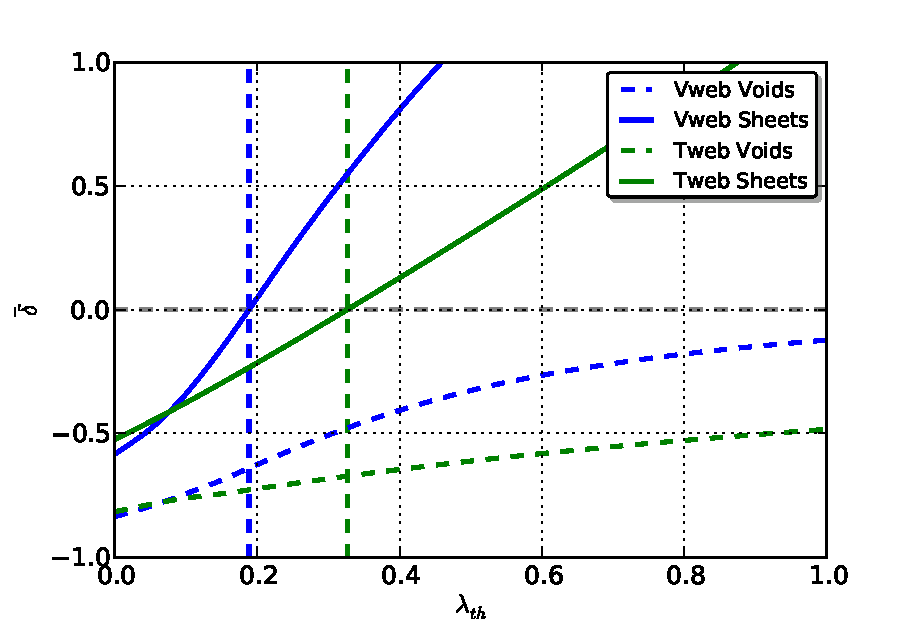
\includegraphics[trim = 0mm 10mm 12mm 19mm, clip, keepaspectratio=true,
  width=0.3\textheight]{./figures/cell_types_density.pdf}

  \captionof{figure}{\small Mean density parameter for each one of the 
  defined environments according to the chosen $\lambda_{th}$ value and 
  for both classification schemes. Tweb (green lines) and Vweb (blue 
  lines). The mean density parameter is calculated by averaging all the 
  values  of the cells determined as a certain type of environment 
  according to its eigenvalues. The optimal parameters found are 
  $\lambda_{opt}^{T}=0.326$ and $\lambda_{opt}^{V}=0.188$.}

  \label{fig:mean_density}
  \vspace{0.1 cm}

\end{center}
\end{figure*}
\end{flushleft}
%.........................................................................



%.........................................................................
%Visual impresion
\begin{flushleft}
\begin{figure*}
\begin{center}

  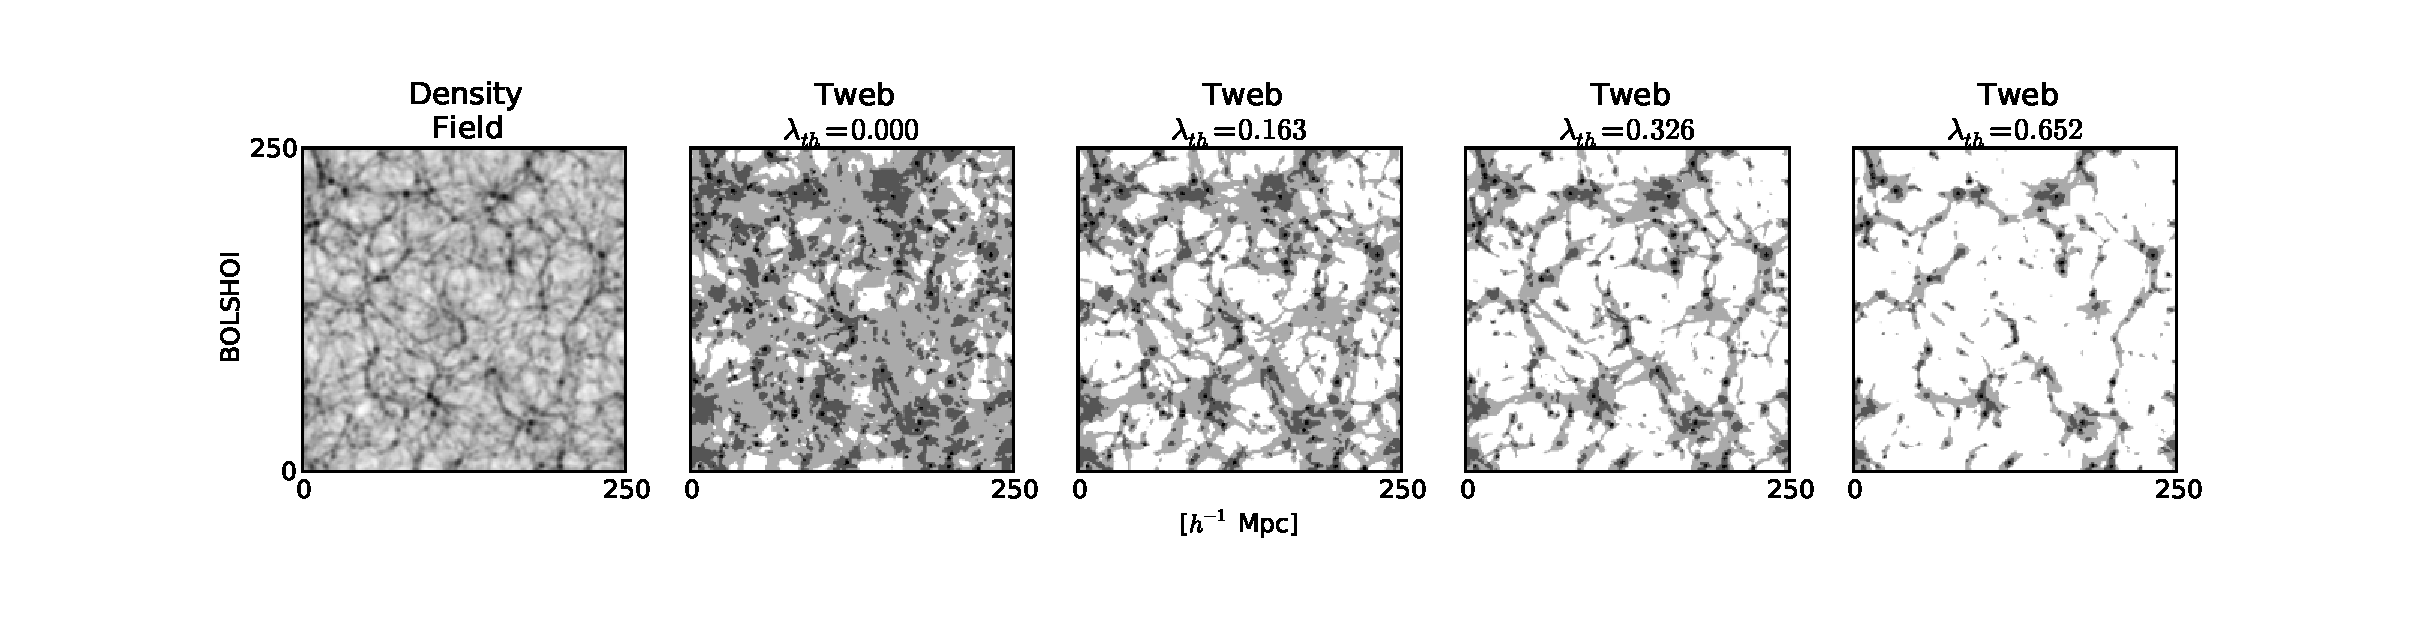
\includegraphics[trim = 42mm 15mm 37mm 10mm, clip, keepaspectratio=true,
  width=0.7\textheight]{./figures/cosmicweb_visual_Tweb.pdf}
  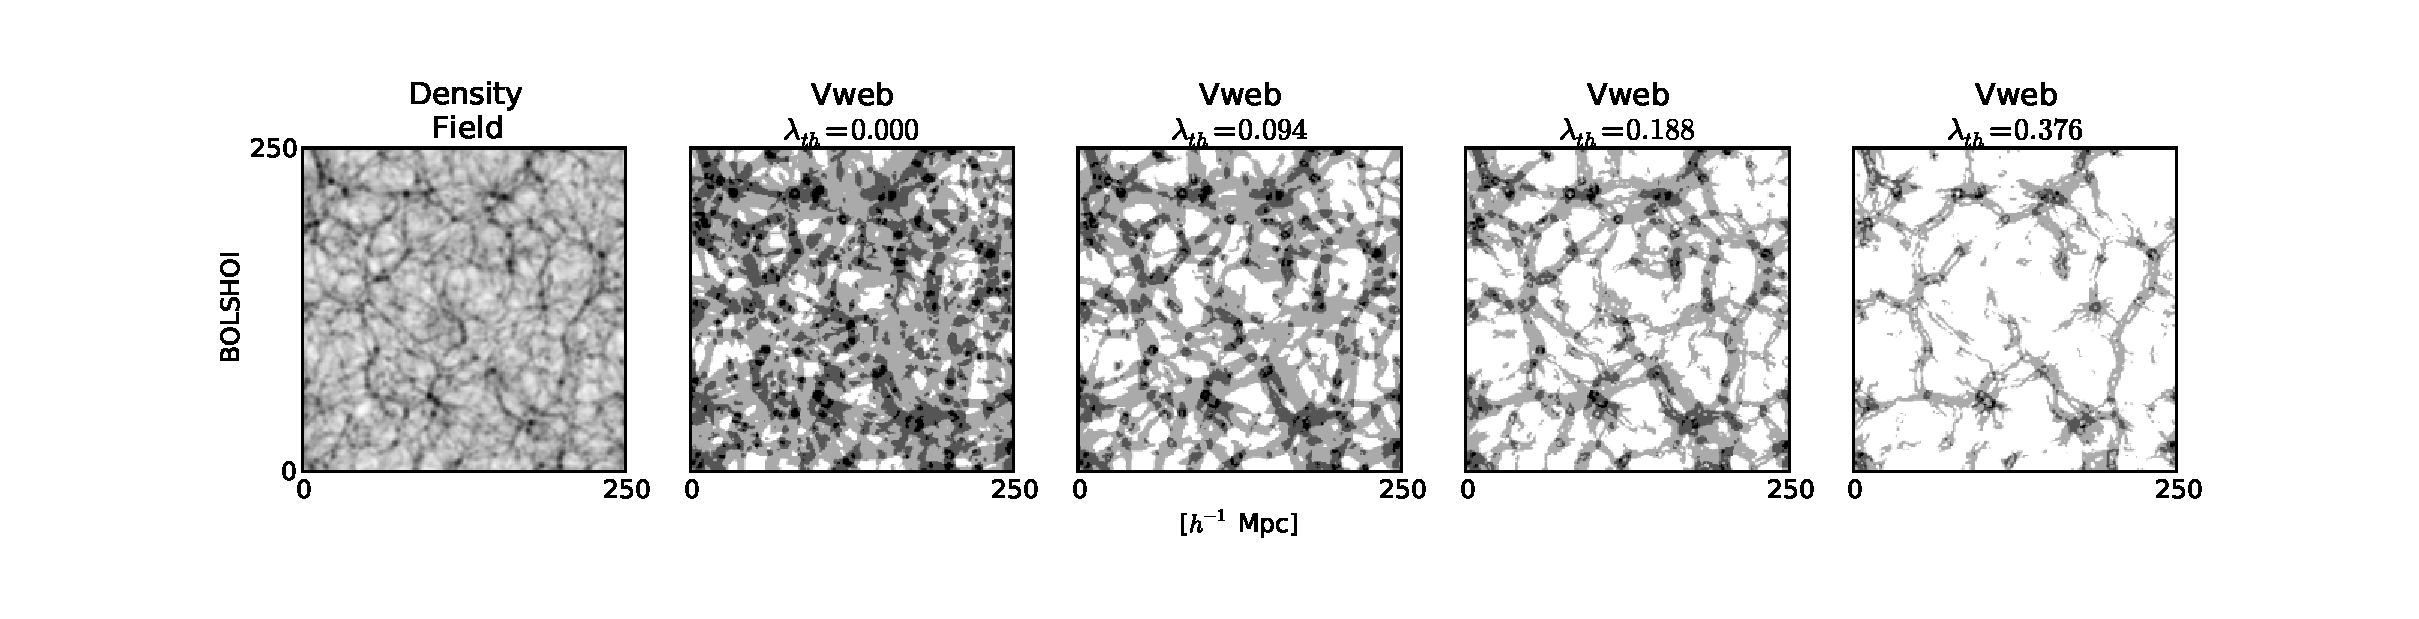
\includegraphics[trim = 42mm 15mm 37mm 10mm, clip, keepaspectratio=true,
  width=0.7\textheight]{./figures/cosmicweb_visual_Vweb.pdf}

  \captionof{figure}{\small Visual impression of the density field (left 
  panels), and of each classification scheme with the $\lambda_{th}$ values 
  obtained by our criteria (others panels). Our color convention for each 
  environment is (white) - void, (light gray) - sheet, (gray) - filament, 
  (black) - knot. For each web scheme, it has been used the previously 
  established optimal threshold as a reference value, so plots are done 
  with the next values $\lambda_{th} = 0.0$, $\lambda_{th} = 
  \lambda_{opt}/2$, $\lambda_{th} = \lambda_{opt}$ and $\lambda_{th} = 
  2\lambda_{opt}$.}

  \label{fig:visual_impression}
  \vspace{0.1 cm}

\end{center}
\end{figure*}
\end{flushleft}
%.........................................................................



%.........................................................................
%Percolation analysis
\begin{flushleft}
\begin{figure*}
\begin{center}

  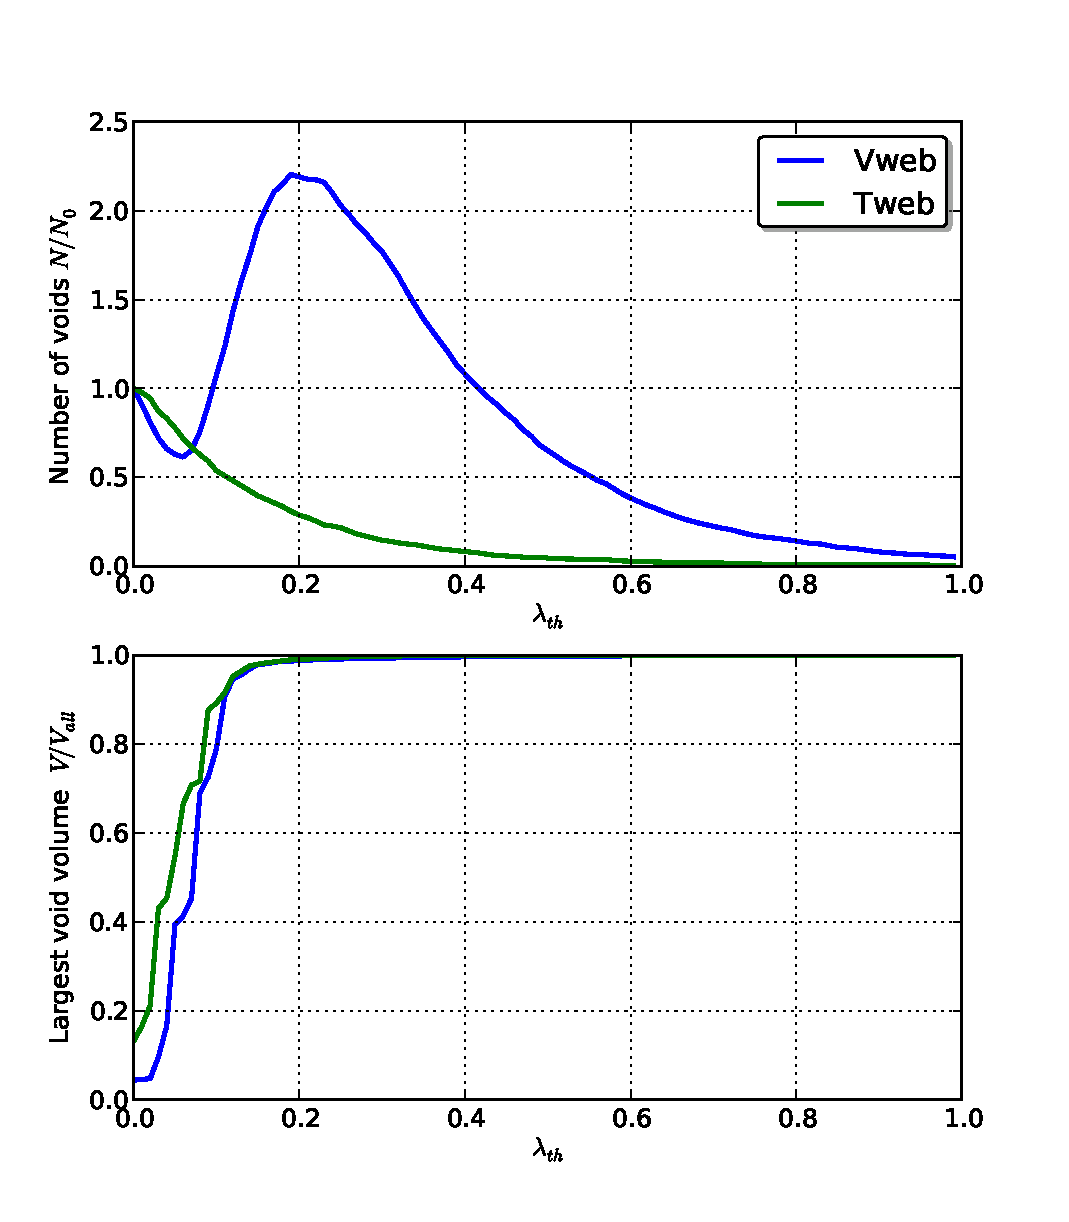
\includegraphics[trim = 1mm 10mm 8mm 18mm, clip, keepaspectratio=true,
  width=0.24\textheight]{./figures/voids_regions_percolation.pdf}
  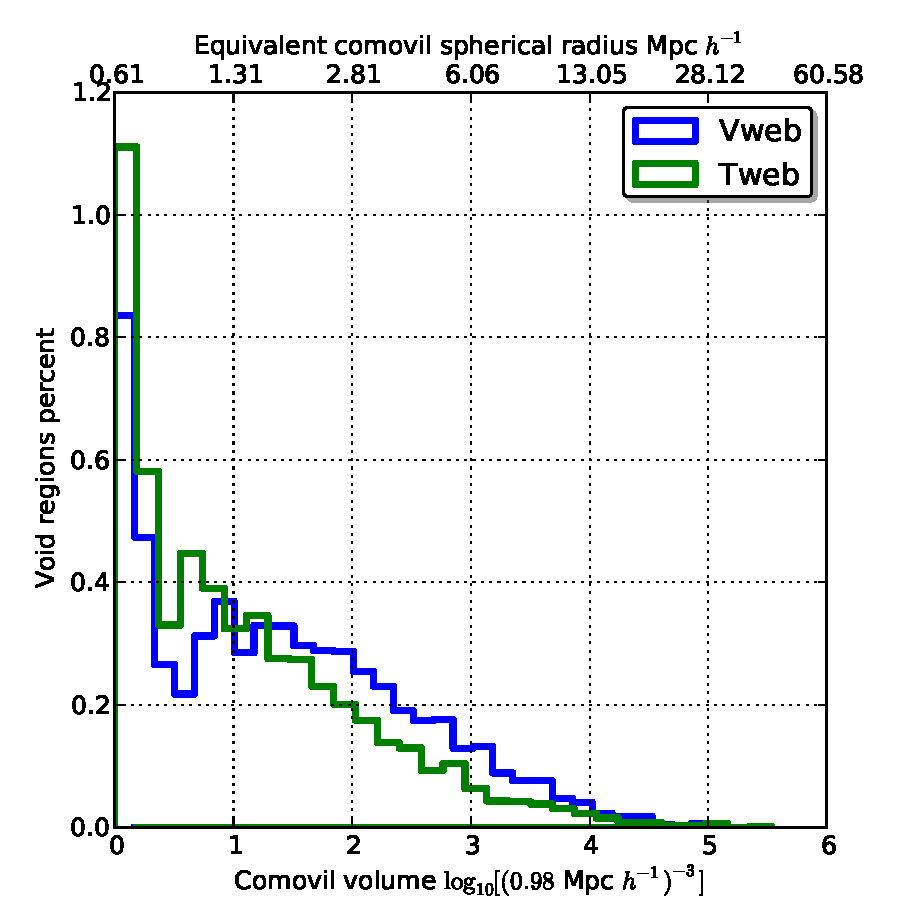
\includegraphics[trim = 0mm 00mm 00mm 00mm, clip, keepaspectratio=true,
  width=0.35\textheight]{./figures/voids_regions_volume.pdf}

  \captionof{figure}{\small Percolation analysis of void regions for 
  different $\lambda_{th}$ values and for both defined classification 
  schemes. T-web (blue lines) and  V-web (green lines). Plot of the largest 
  volume and the number of voids detected according to the threshold value 
  $\lambda_{th}$ (left panels). Size distribution histogram of void cells
  using the threshold value $\lambda_{th} = 0.0$ for both schemes 
  (right panel).}

  \label{fig:percolation_analysis}
  \vspace{0.1 cm}

\end{center}
\end{figure*}
\end{flushleft}
%.........................................................................



%.........................................................................
%Distribution of eigenvalues of the inertia tensor
\begin{flushleft}
\begin{figure*}
\begin{center}

  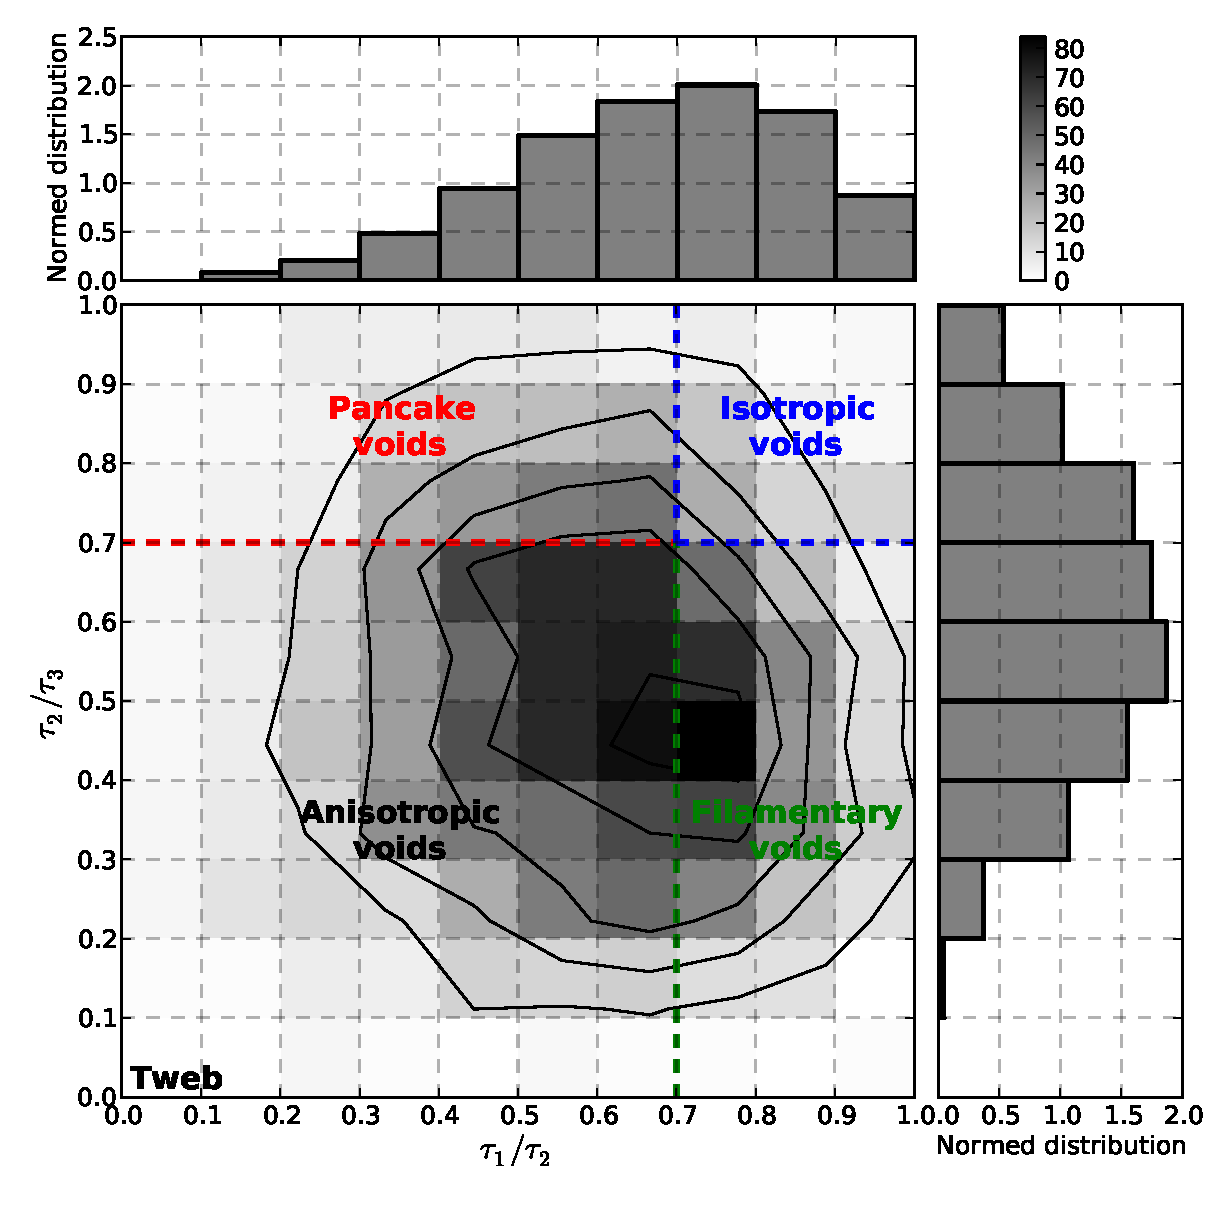
\includegraphics[trim = 7mm 9mm 1mm 0mm, clip, keepaspectratio=true,
  width=0.36\textheight]{./figures/voids_inertia_tensor_Tweb}
  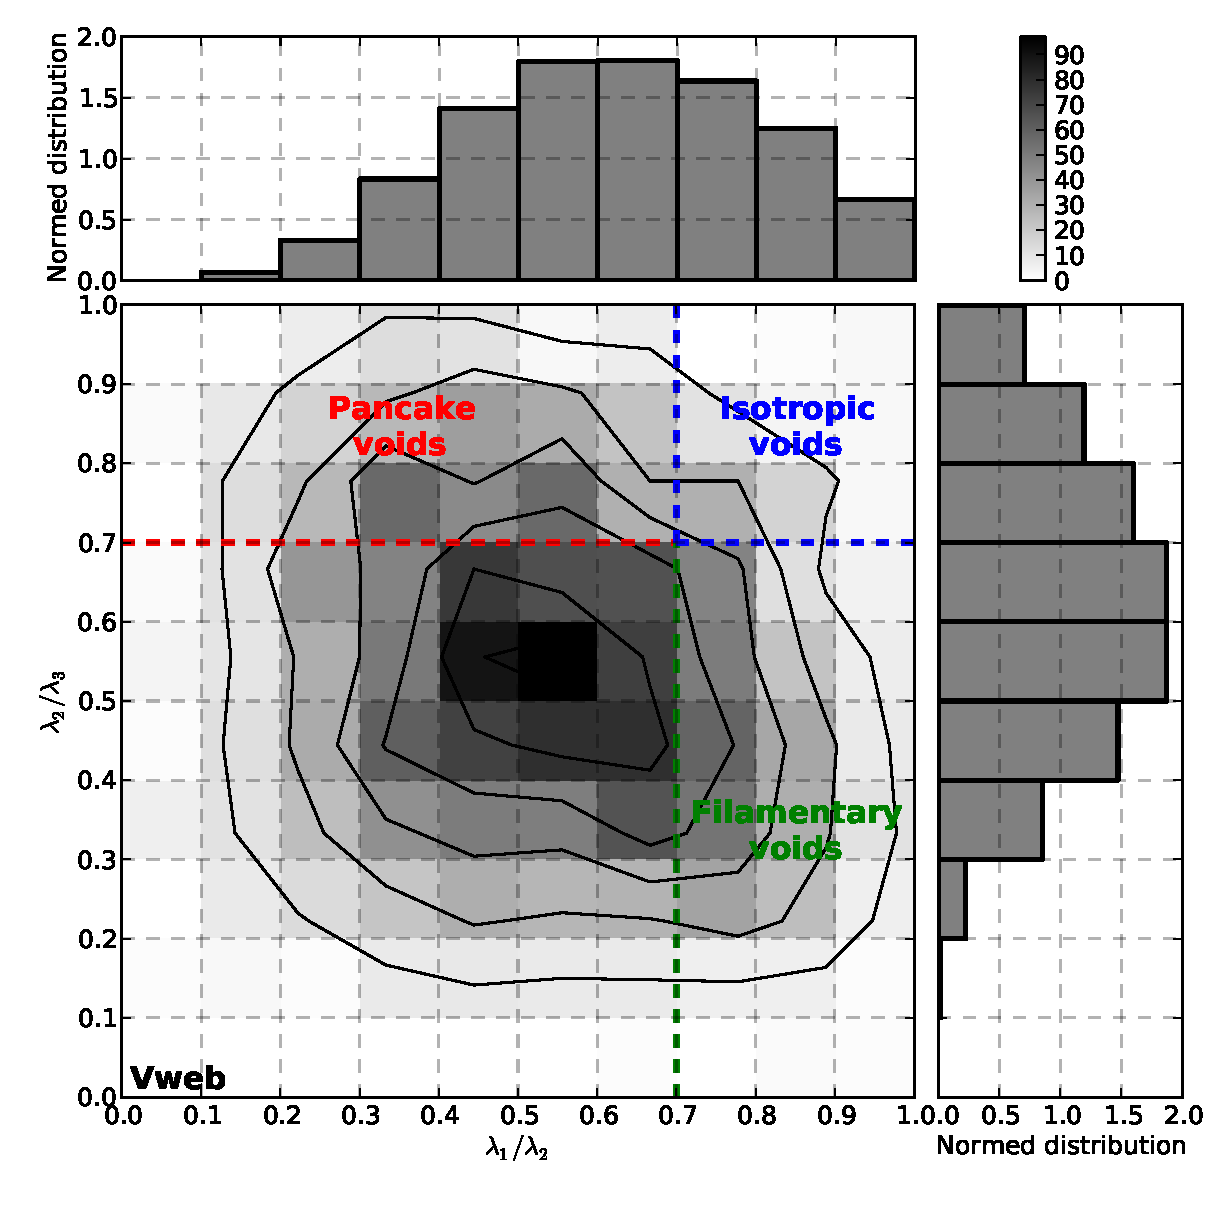
\includegraphics[trim = 7mm 9mm 1mm 0mm, clip, keepaspectratio=true,
  width=0.36\textheight]{./figures/voids_inertia_tensor_Vweb}

  \captionof{figure}{\small Histogram of eigenvalue ratio $\tau_1/\tau_2$
  vs $\tau_2/\tau_3$ for the inertia tensor of void regions. T-web 
  (left panel) and V-web (right panel). Number of cells per 
  region in 2D histograms are indicated by the respective colour bar. 
  Upper ($\tau_1/\tau_2$) and right ($\tau_2/\tau_3$) panels of each 
  figure shows a normalized histogram of each ratio parameter. The 
  adopted division for quantify the morphology of void regions is not
  a well justified, it must be understood as a fuzzy and continuous 
  limit, done just for illustrative purposes.}

  \label{fig:distro_inertia}
  \vspace{0.1 cm}

\end{center}
\end{figure*}
\end{flushleft}
%.........................................................................



%.........................................................................
%Distribution of eigenvalues of the web schemes
\begin{flushleft}
\begin{figure*}
\begin{center}

  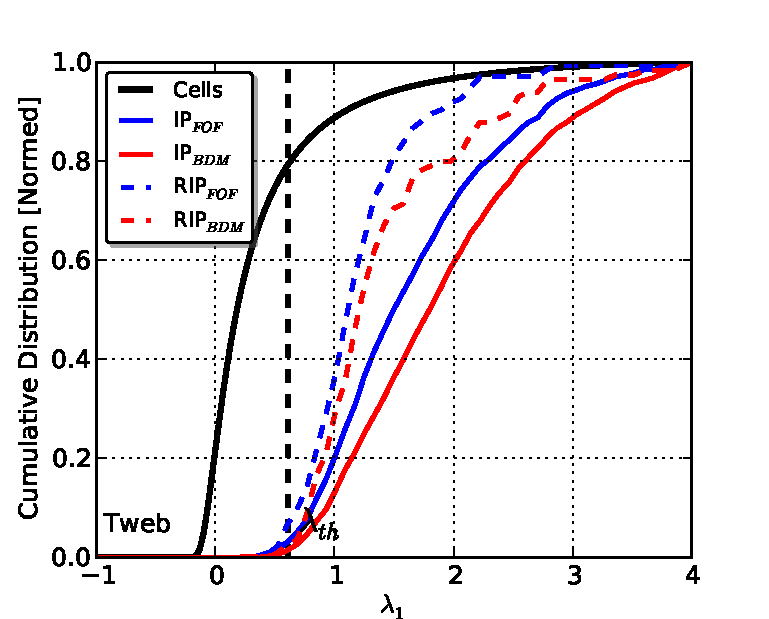
\includegraphics[trim = 3mm 0mm 10mm 8mm, clip, keepaspectratio=true,
  width=0.24\textheight]{./figures/eigen1_dist_Tweb}
  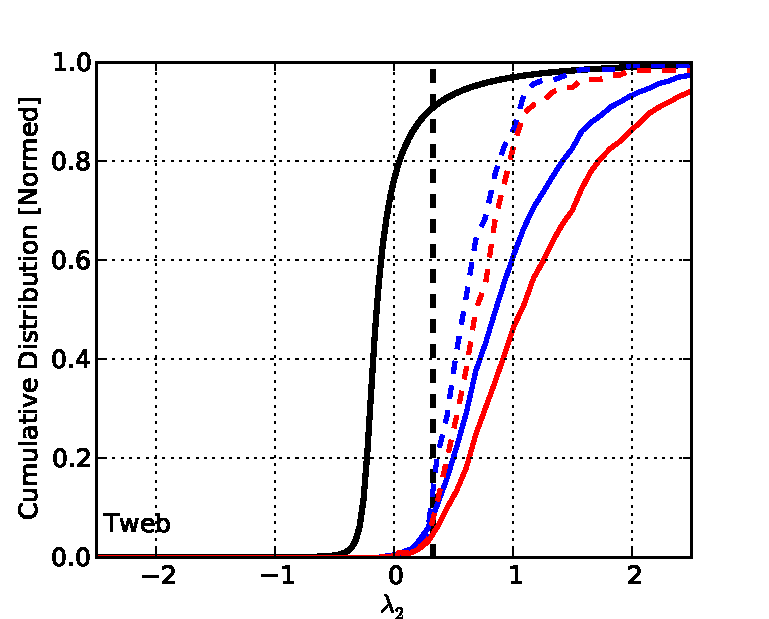
\includegraphics[trim = 3mm 0mm 10mm 8mm, clip, keepaspectratio=true,
  width=0.24\textheight]{./figures/eigen2_dist_Tweb}
  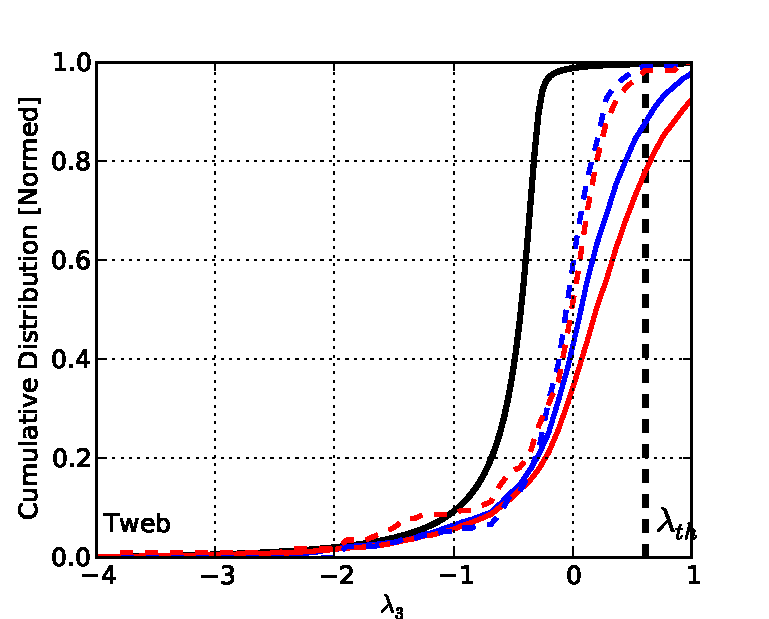
\includegraphics[trim = 3mm 0mm 10mm 8mm, clip, keepaspectratio=true,
  width=0.24\textheight]{./figures/eigen3_dist_Tweb}

  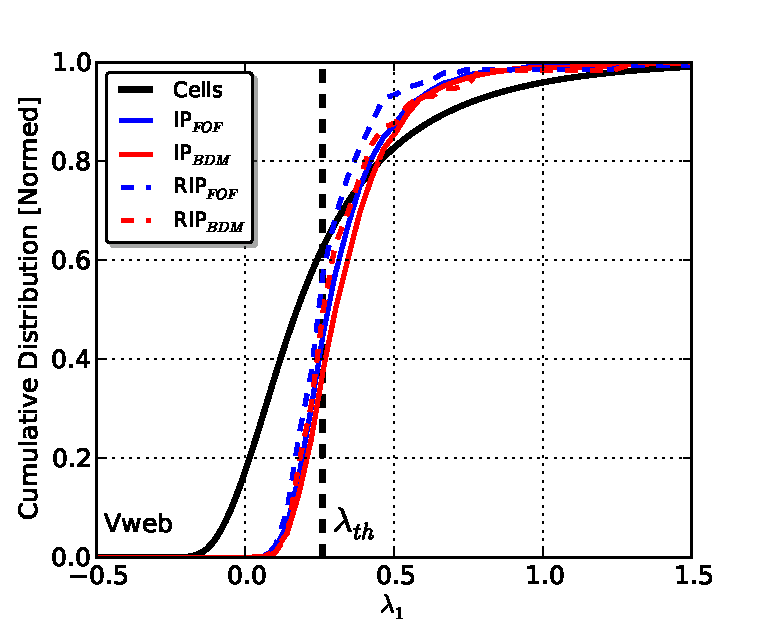
\includegraphics[trim = 3mm 0mm 10mm 8mm, clip, keepaspectratio=true,
  width=0.24\textheight]{./figures/eigen1_dist_Vweb}
  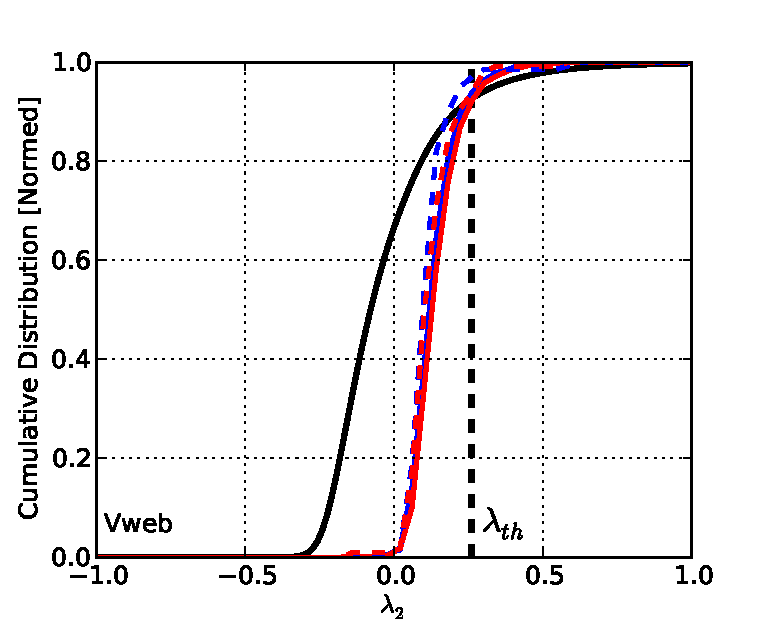
\includegraphics[trim = 3mm 0mm 10mm 8mm, clip, keepaspectratio=true,
  width=0.24\textheight]{./figures/eigen2_dist_Vweb}
  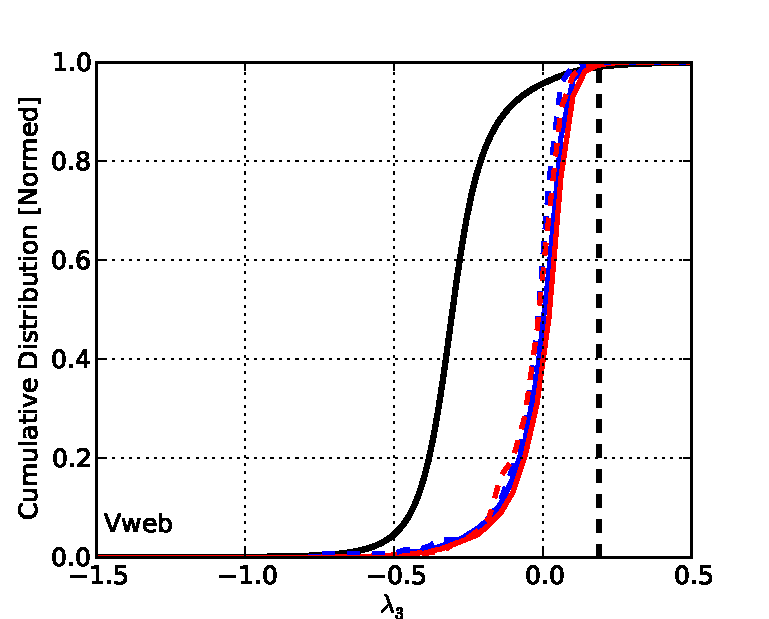
\includegraphics[trim = 3mm 0mm 10mm 8mm, clip, keepaspectratio=true,
  width=0.24\textheight]{./figures/eigen3_dist_Vweb}
  
  \captionof{figure}{\small Distributions of eigenvalues for each defined
  scheme. T-web (upper panels) and V-web (lower panels). In each figure is
  calculated the distributions of eigenvalues for the volume cells of the 
  simulation (black lines), evaluating the respective tensor on the 
  geometric center of the cell. This is also done for \texttt{IP} 
  (continuous lines) and \texttt{RIP} (dashed lines) samples (both BDM 
  (red) and FOF (blue)), but the tensors are evaluated on the cell which 
  contains the center of mass of the halo pair. The vertical dashed line
  corresponds to the optimal threshold value $\lambda_{opt}$ for each 
  scheme respectively.}

  \label{fig:distro_cosmicweb}
  \vspace{0.1 cm}

\end{center}
\end{figure*}
\end{flushleft}
%.........................................................................



%.........................................................................
%Distribution of fractional anisotropy
\begin{flushleft}
\begin{figure*}
\begin{center}

  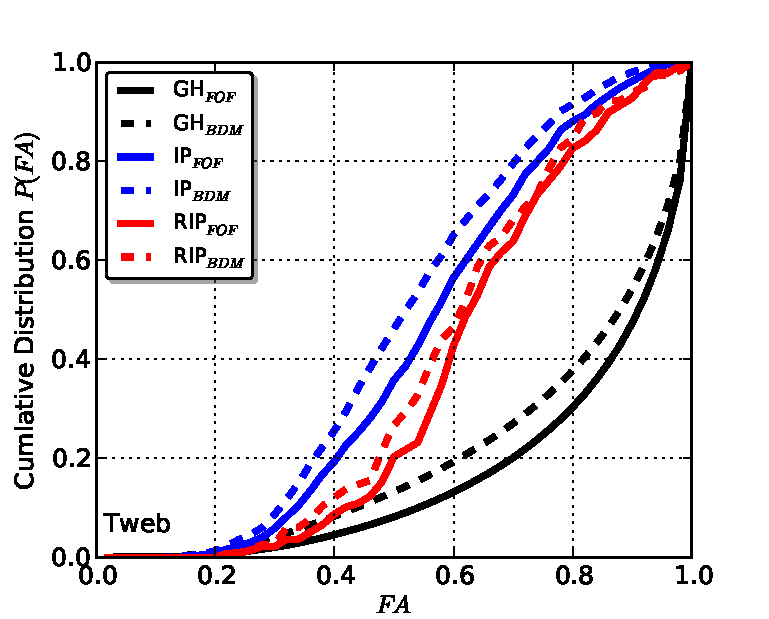
\includegraphics[trim = 0mm 0mm 0mm 0mm, clip, keepaspectratio=true,
  width=0.3\textheight]{./figures/fractional_anisotrpy_Tweb}
  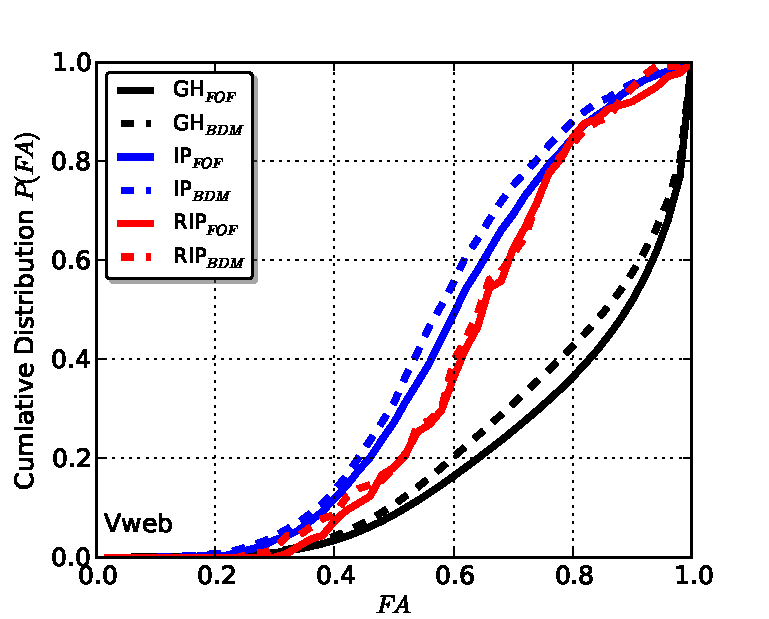
\includegraphics[trim = 0mm 0mm 0mm 0mm, clip, keepaspectratio=true,
  width=0.3\textheight]{./figures/fractional_anisotrpy_Vweb}
  
  \captionof{figure}{\small Cumulative distribution of the fractional 
  anisotropy for each web scheme. T-web (right panel) and V-web (left panel).
  Distributions for each sample are also calculated, \texttt{GH} sample 
  (black lines), \texttt{IP} sample (blue lines) and \texttt{RIP} sample 
  (red lines). In order to compare each halo scheme, we also calculate 
  distributions for each one, FOF (dashed lines) and BDM (continuous 
  lines). }

  \label{fig:fractional_anisotropy}
  \vspace{0.1 cm}

\end{center}
\end{figure*}
\end{flushleft}
%.........................................................................



%.........................................................................
%Distribution of size and distance to void regions respect to each sample
\begin{flushleft}
\begin{figure*}
\begin{center}

  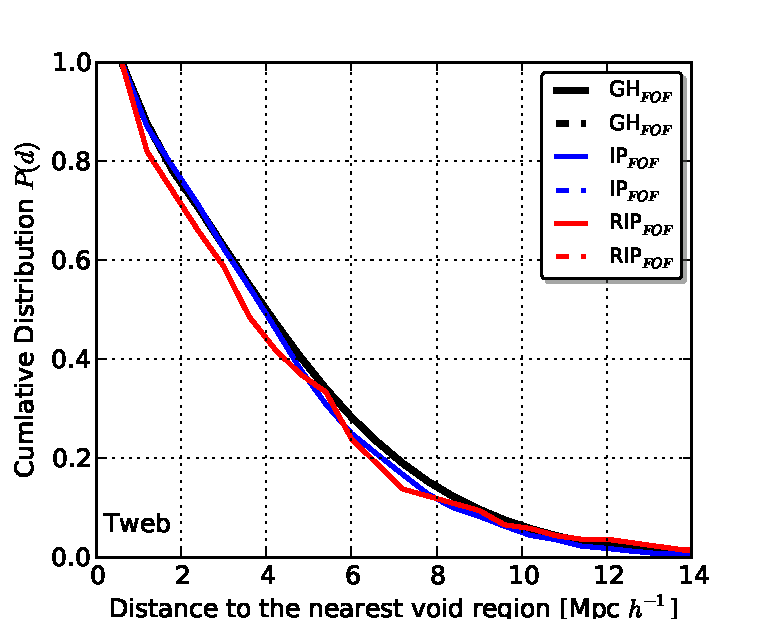
\includegraphics[trim = 0mm 0mm 0mm 0mm, clip, keepaspectratio=true,
  width=0.3\textheight]{./figures/voids_distances_samples_Tweb}
  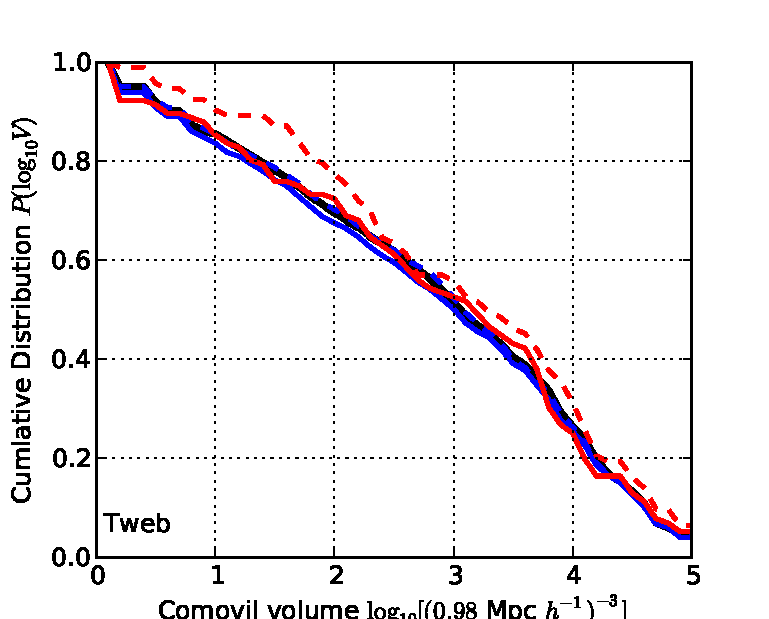
\includegraphics[trim = 0mm 0mm 0mm 0mm, clip, keepaspectratio=true,
  width=0.3\textheight]{./figures/voids_sizes_samples_Tweb}
  
  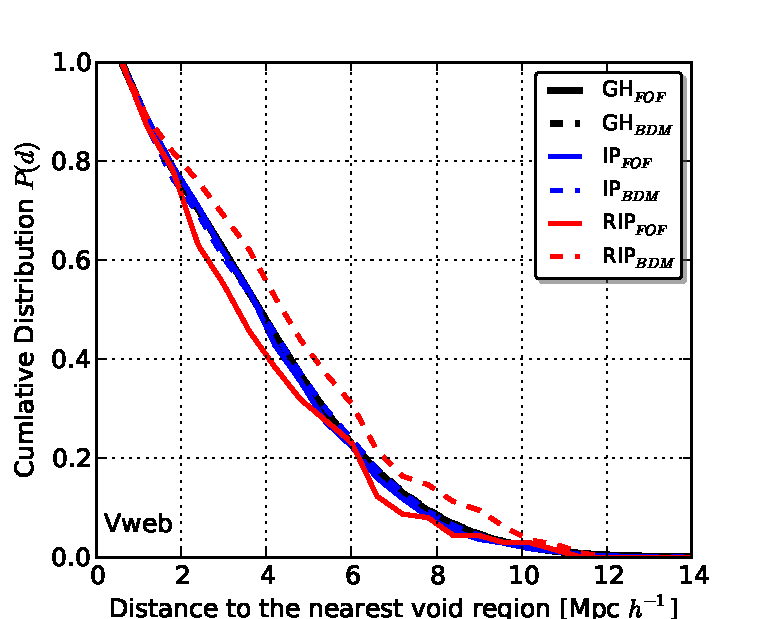
\includegraphics[trim = 0mm 0mm 0mm 0mm, clip, keepaspectratio=true,
  width=0.3\textheight]{./figures/voids_distances_samples_Vweb}
  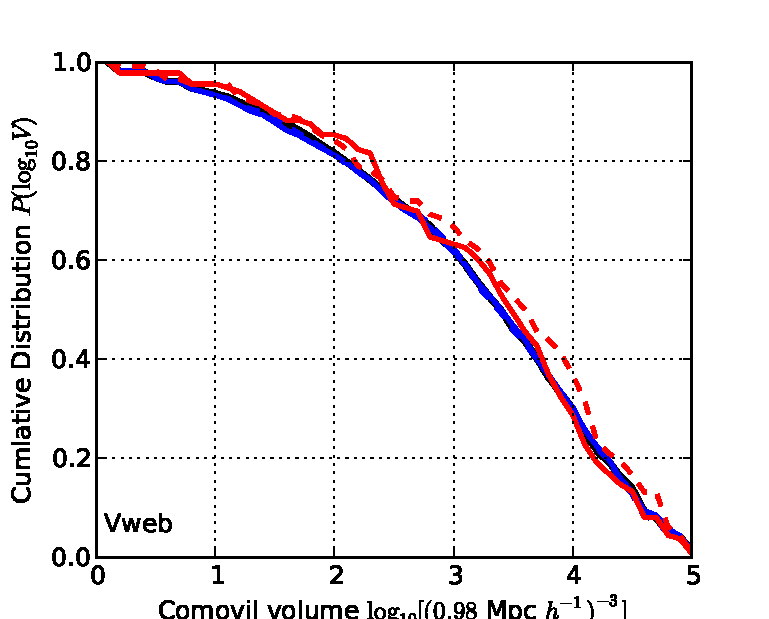
\includegraphics[trim = 0mm 0mm 0mm 0mm, clip, keepaspectratio=true,
  width=0.3\textheight]{./figures/voids_sizes_samples_Vweb}
  
  \captionof{figure}{\small Cumulative distribution of distances (right 
  panels) and volume sizes (left panels) of the nearest void region of 
  each system and for each web scheme. T-web (upper panels) and V-web 
  (lower panels). Systems of the \texttt{GH} sample (black lines), 
  \texttt{IP} sample (blue lines) and \texttt{RIP} sample (red lines) are 
  considered. It is also included both halo schemes, FOF (dashed lines) and 
  BDM (continuous lines).}

  \label{fig:voids2samples}
  \vspace{0.1 cm}

\end{center}
\end{figure*}
\end{flushleft}
%.........................................................................



%.........................................................................
%Distributions of the total mass of pair systems vs the respective FA value
\begin{flushleft}
\begin{figure*}
\begin{center}

  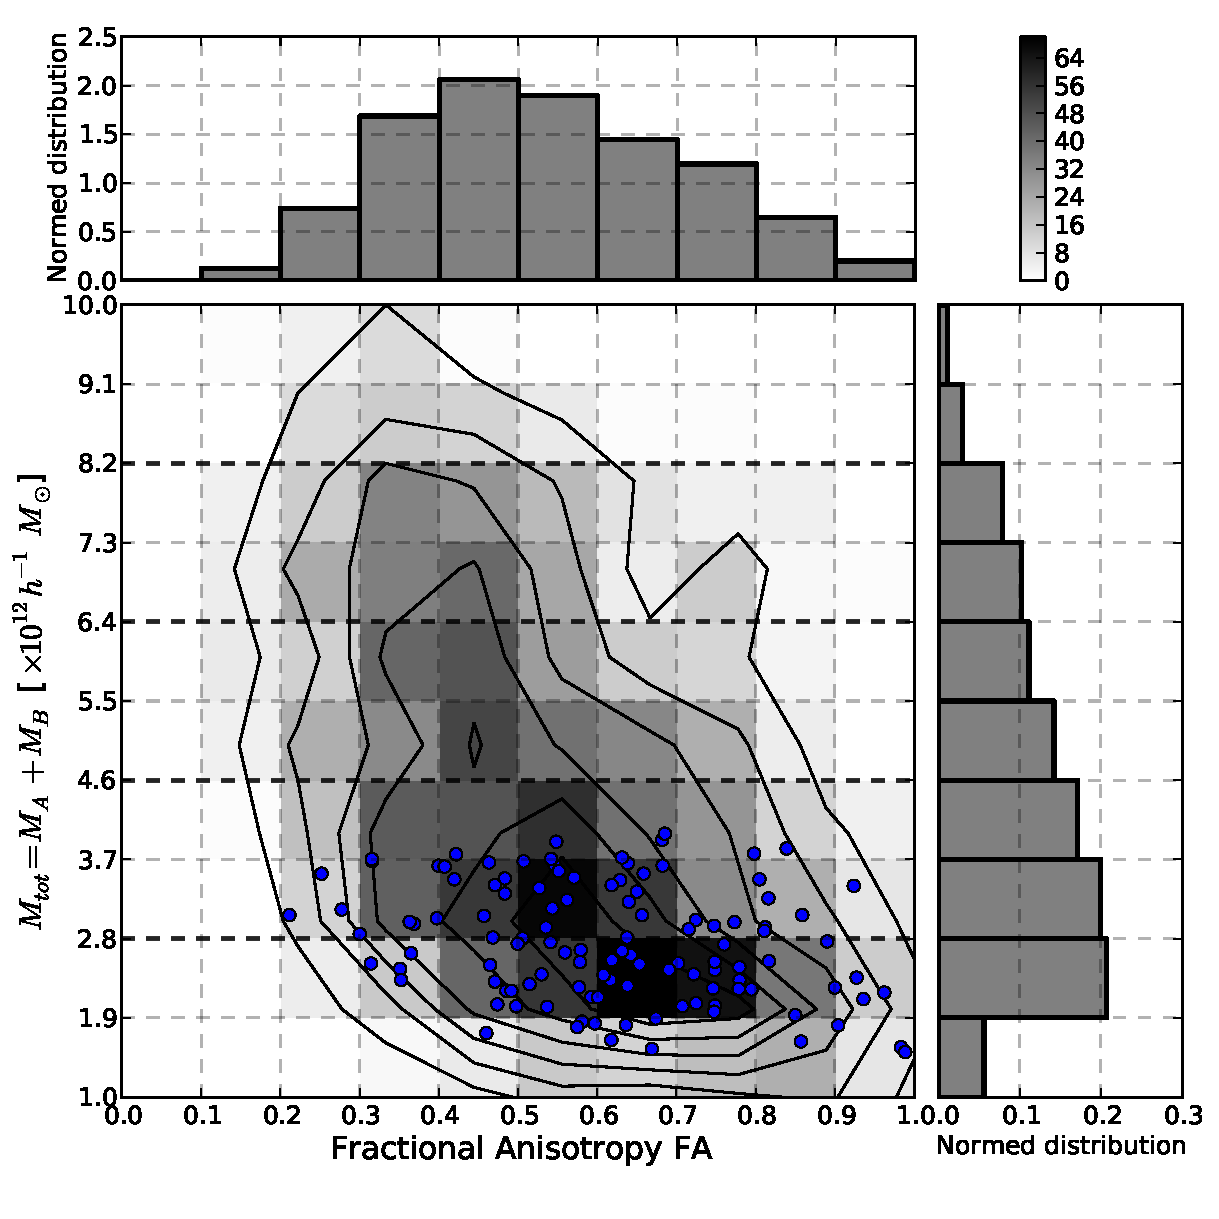
\includegraphics[trim = 2mm 9mm 3mm 4mm, clip, keepaspectratio=true,
  width=0.36\textheight]{./figures/2D_totalmass_FA_BDM_Tweb}
  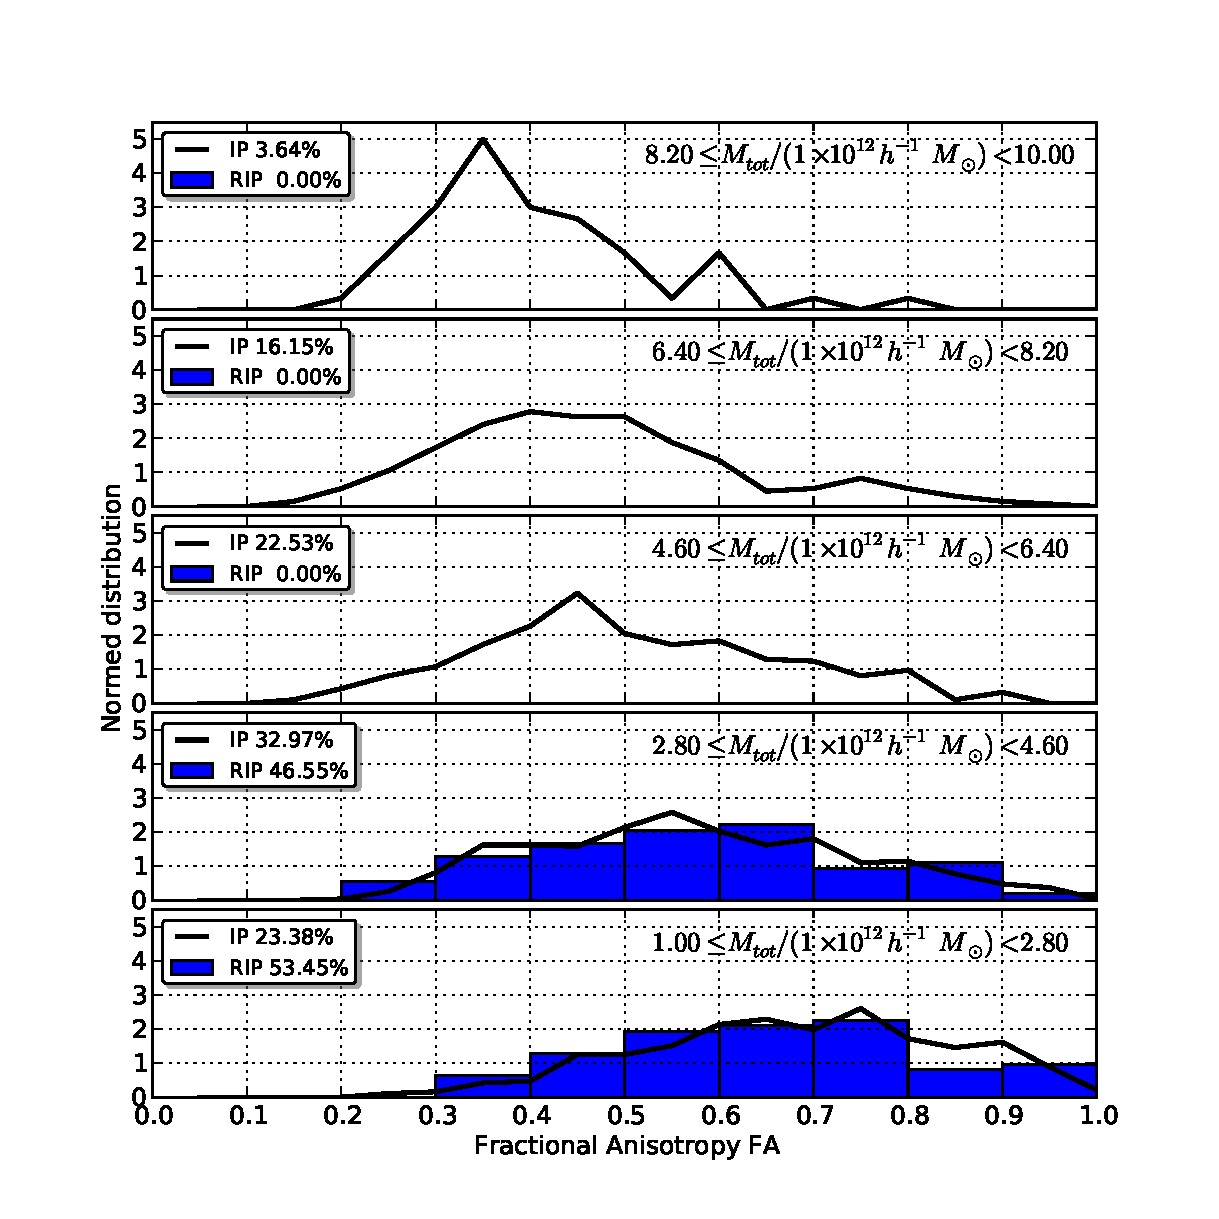
\includegraphics[trim = 4mm 9mm 17mm 15mm, clip, keepaspectratio=true,
  width=0.36\textheight]{./figures/single_totalmass_FA_BDM_Tweb}
  
  \captionof{figure}{\small \textit{Left panel:} histograms of the total 
  mass of each pair sample, \texttt{IP} (2D histogram) and \texttt{RIP} 
  (blue scatter), vs the fractional anisotropy index associated to each 
  system. In the side panels we compute individual histograms of each one 
  of the analysed properties for \texttt{IP} systems. \textit{Right 
  panel:} selecting different mass ranges for the total mass of the pairs, 
  specified in each single panel, we calculate histograms of the 
  fractional anisotropy of each sample, \texttt{IP} (black lines) and 
  \texttt{RIP} (blue bars).}

  \label{fig:totalmass_FA}
  \vspace{0.1 cm}

\end{center}
\end{figure*}
\end{flushleft}
%.........................................................................



%.........................................................................
%Distributions of the total mass of pair systems vs the respective 
%void distance
\begin{flushleft}
\begin{figure*}
\begin{center}

  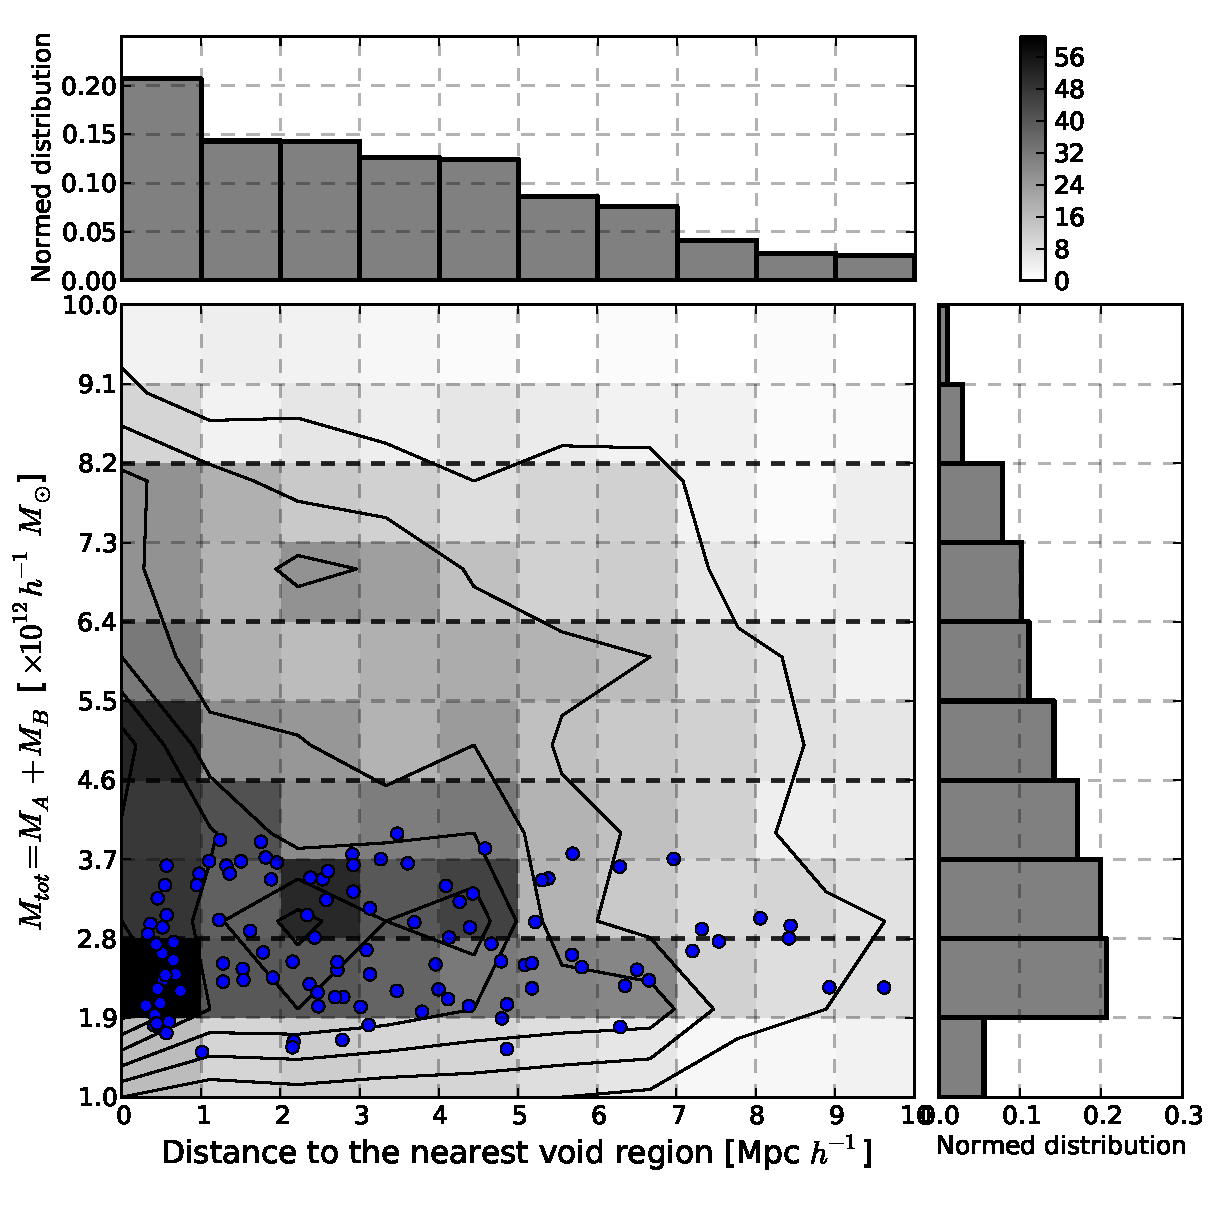
\includegraphics[trim = 2mm 9mm 3mm 4mm, clip, keepaspectratio=true,
  width=0.36\textheight]{./figures/2D_totalmass_vdistance_BDM_Tweb}
  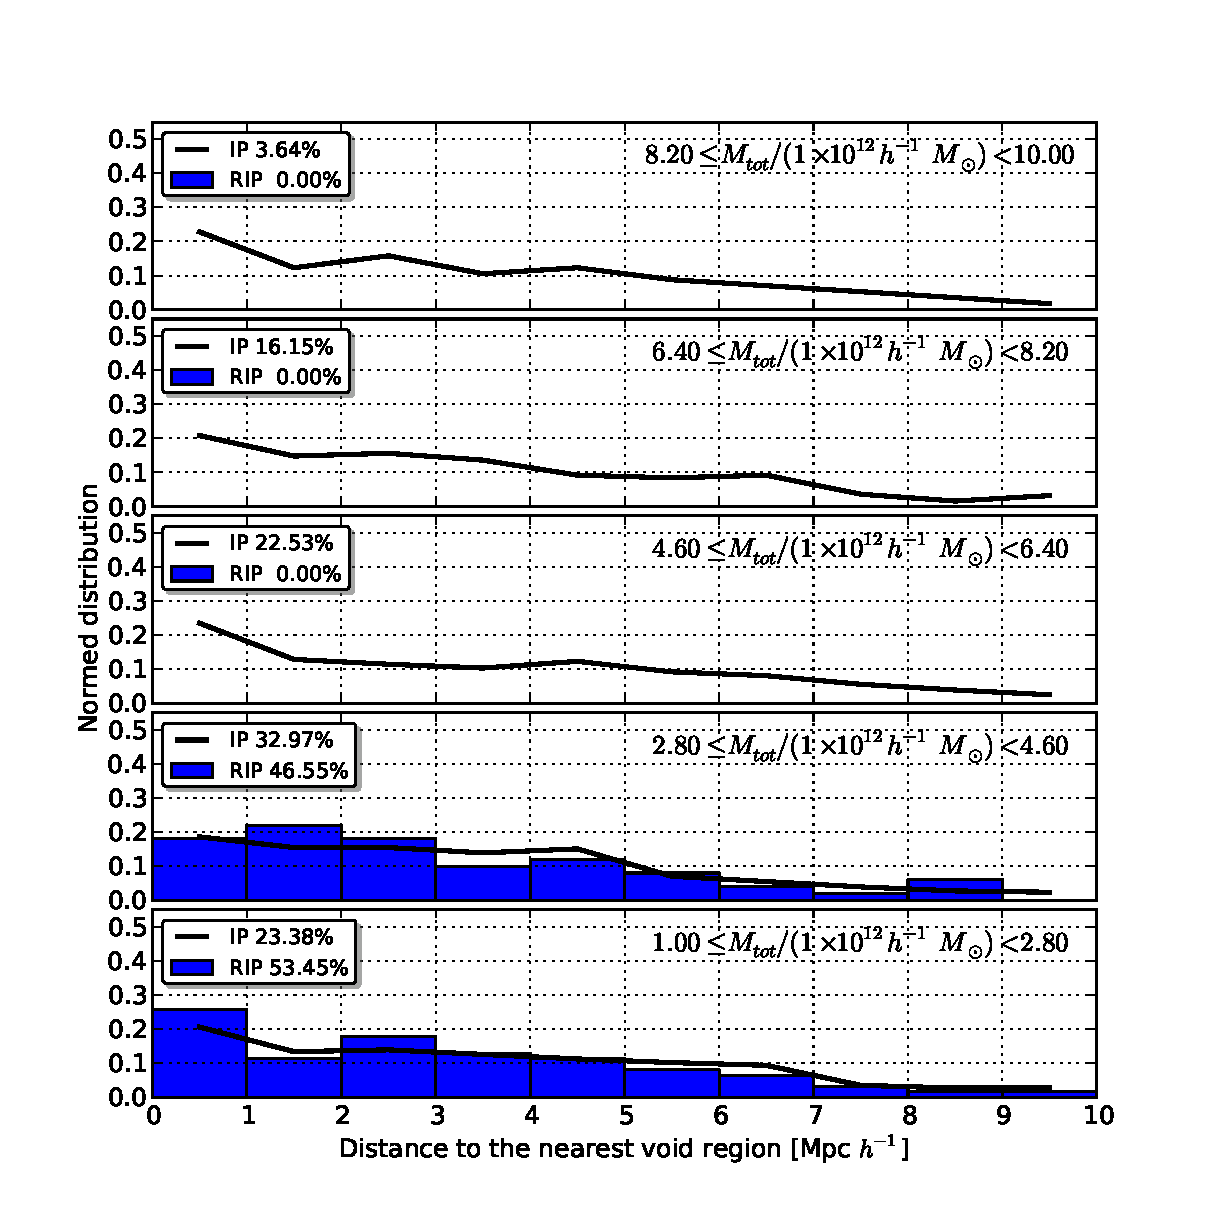
\includegraphics[trim = 4mm 9mm 17mm 15mm, clip, keepaspectratio=true,
  width=0.36\textheight]{./figures/single_totalmass_vdistance_BDM_Tweb}
  
  \captionof{figure}{\small \textit{Left panel:} histograms of the total 
  mass of each pair sample, \texttt{IP} (2D histogram) and \texttt{RIP} 
  (blue scatter), vs the distance to the nearest void region associated to 
  each system. In the side panels we compute individual histograms of each one 
  of the analysed properties for \texttt{IP} systems. \textit{Right 
  panel:} selecting different ranges for the mass ratio of the pairs, 
  specified in each single panel, we calculate histograms of the 
  distance of each sample, \texttt{IP} (black lines) and 
  \texttt{RIP} (blue bars).}

  \label{fig:totalmass_vdistance}
  \vspace{0.1 cm}

\end{center}
\end{figure*}
\end{flushleft}
%.........................................................................



%.........................................................................
%Distributions of the total mass of pair systems vs the respective void
%volume
\begin{flushleft}
\begin{figure*}
\begin{center}

  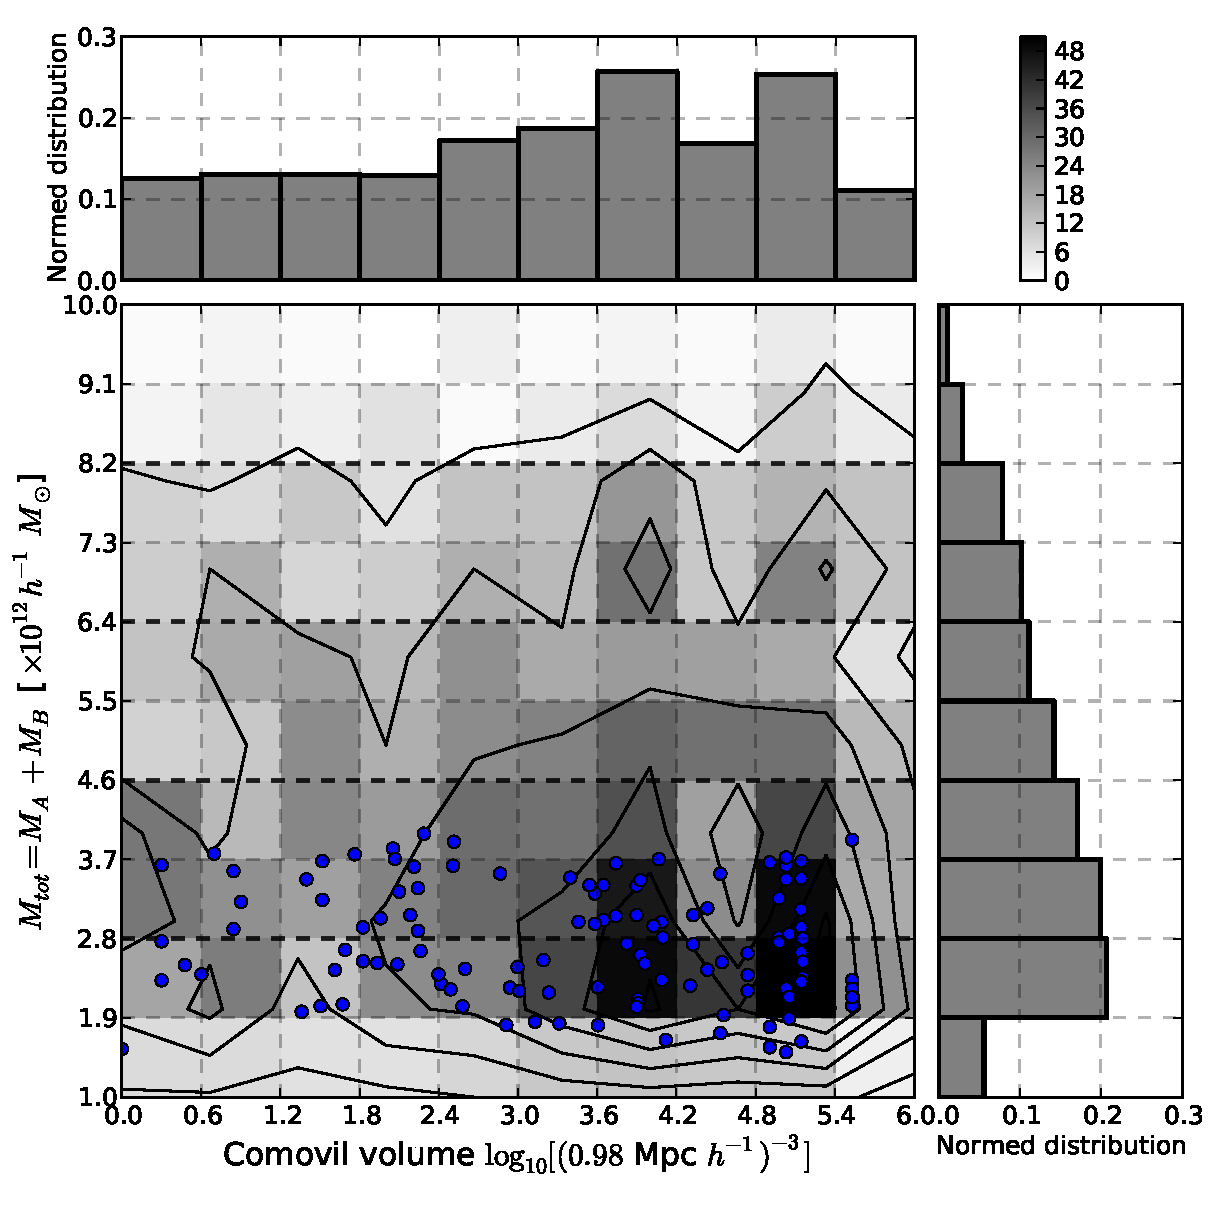
\includegraphics[trim = 2mm 9mm 3mm 4mm, clip, keepaspectratio=true,
  width=0.36\textheight]{./figures/2D_totalmass_vvolume_BDM_Tweb}
  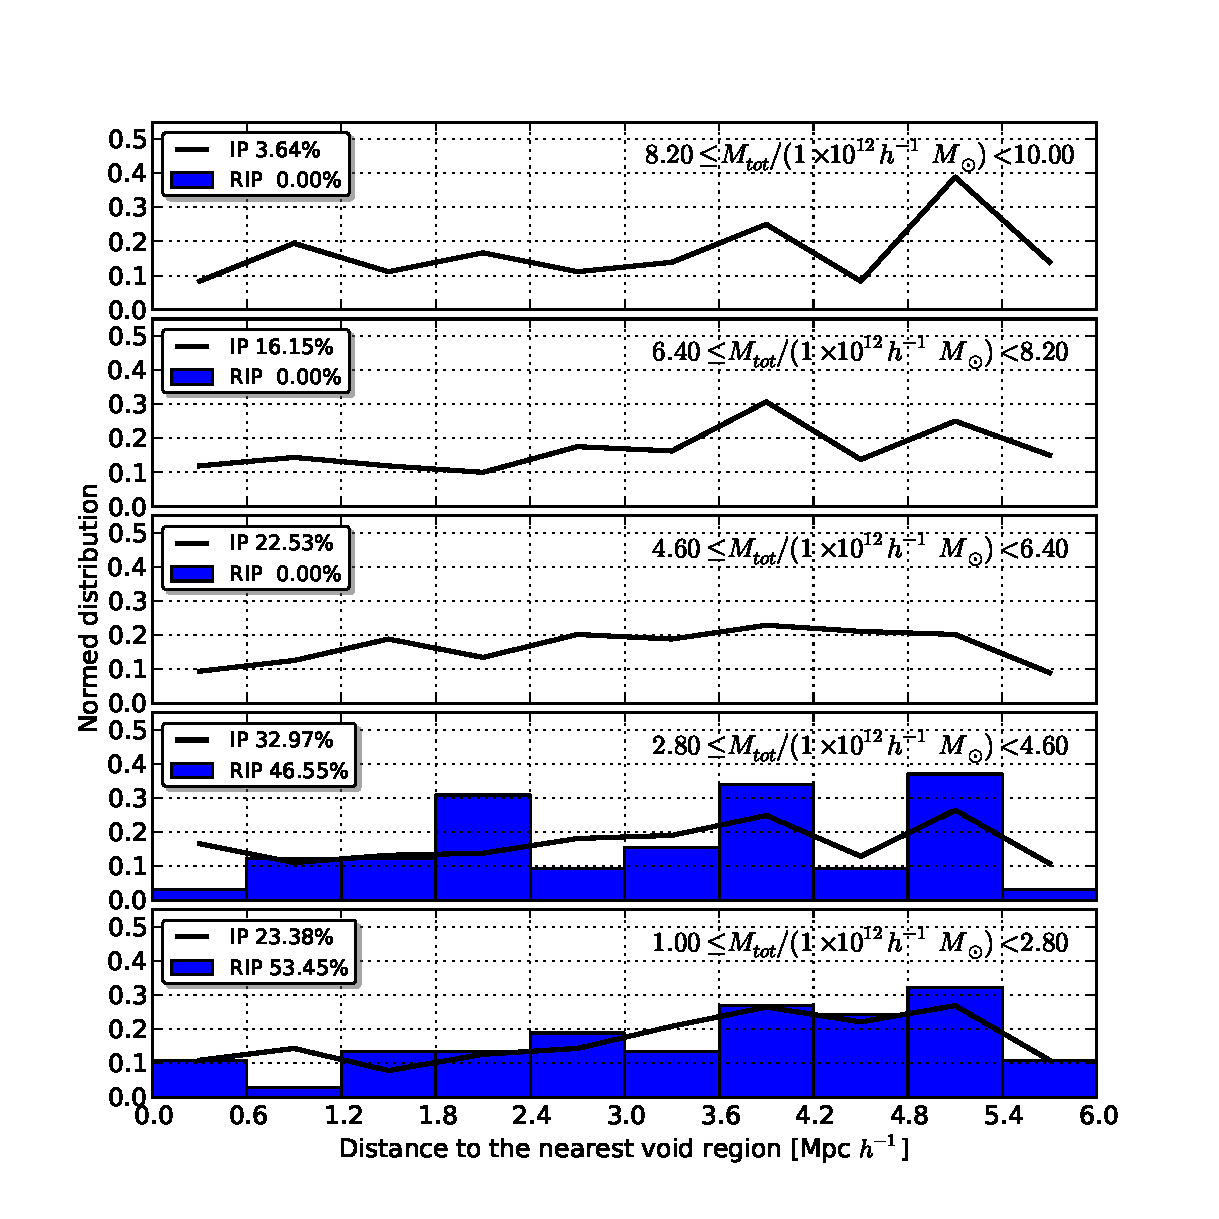
\includegraphics[trim = 4mm 9mm 17mm 15mm, clip, keepaspectratio=true,
  width=0.36\textheight]{./figures/single_totalmass_vvolume_BDM_Tweb}
  
  \captionof{figure}{\small \textit{Left panel:} histograms of the total 
  mass of each pair sample, \texttt{IP} (2D histogram) and \texttt{RIP} 
  (blue scatter), vs the distance to the nearest void region associated to 
  each system. In the side panels we compute individual histograms of each one 
  of the analysed properties for \texttt{IP} systems. \textit{Right 
  panel:} selecting different ranges for the mass ratio of the pairs, 
  specified in each single panel, we calculate histograms of the 
  distance of each sample, \texttt{IP} (black lines) and 
  \texttt{RIP} (blue bars).}

  \label{fig:totalmass_vvolume}
  \vspace{0.1 cm}

\end{center}
\end{figure*}
\end{flushleft}
%.........................................................................



%.........................................................................
%Distributions of the radial velocity of pair systems vs the respective 
%FA value
\begin{flushleft}
\begin{figure*}
\begin{center}

  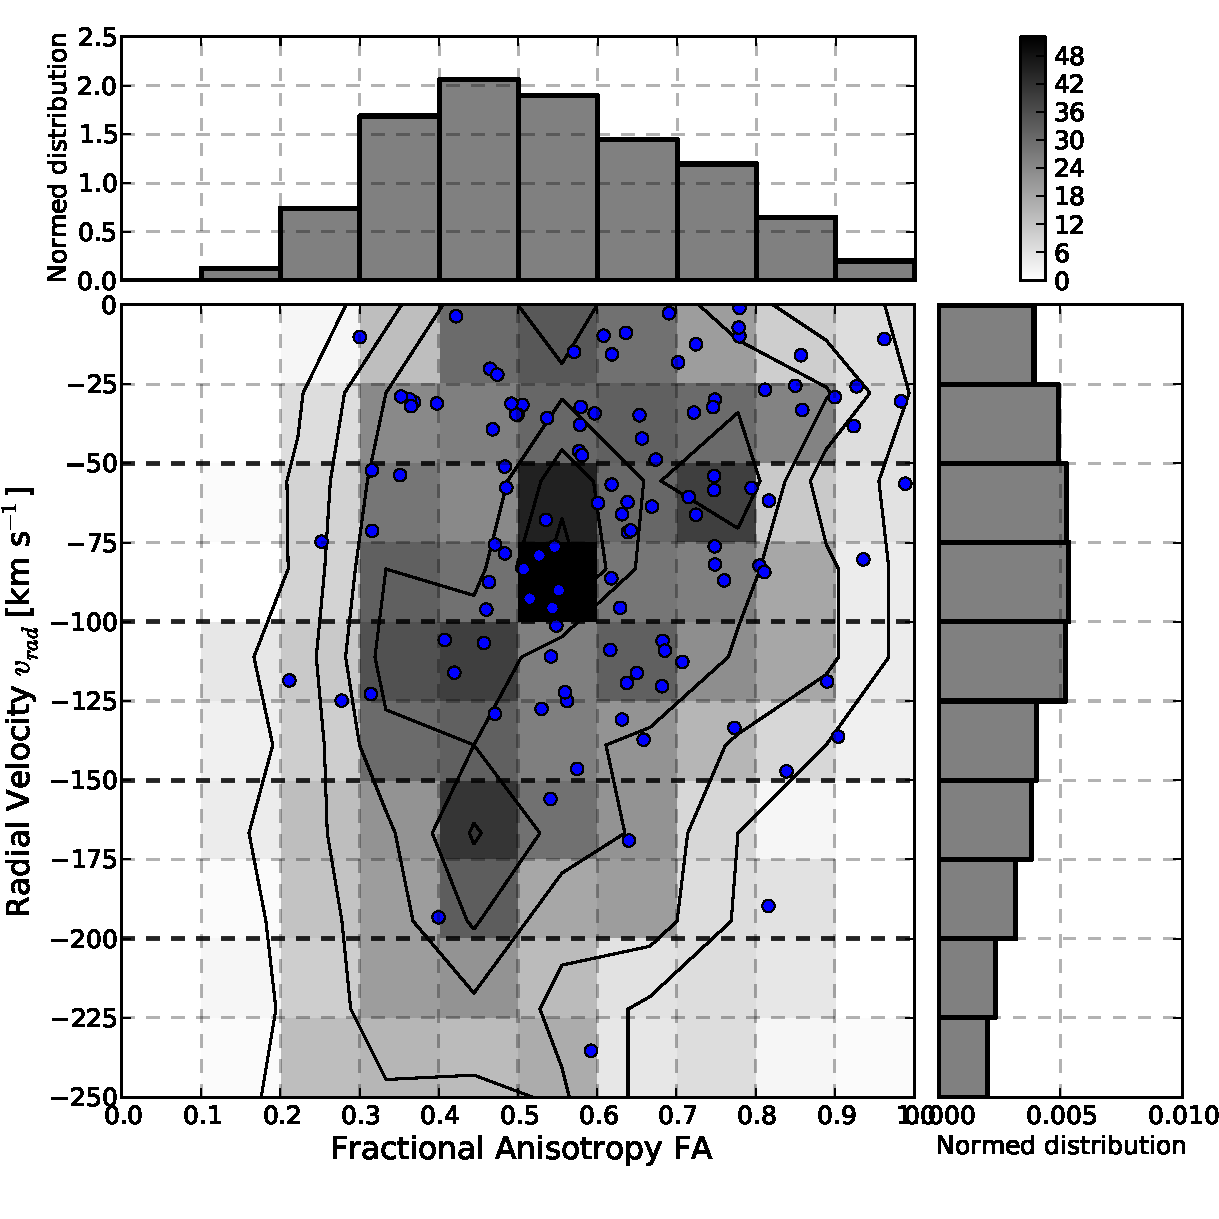
\includegraphics[trim = 2mm 9mm 3mm 4mm, clip, keepaspectratio=true,
  width=0.36\textheight]{./figures/2D_radialvelocity_FA_BDM_Tweb}
  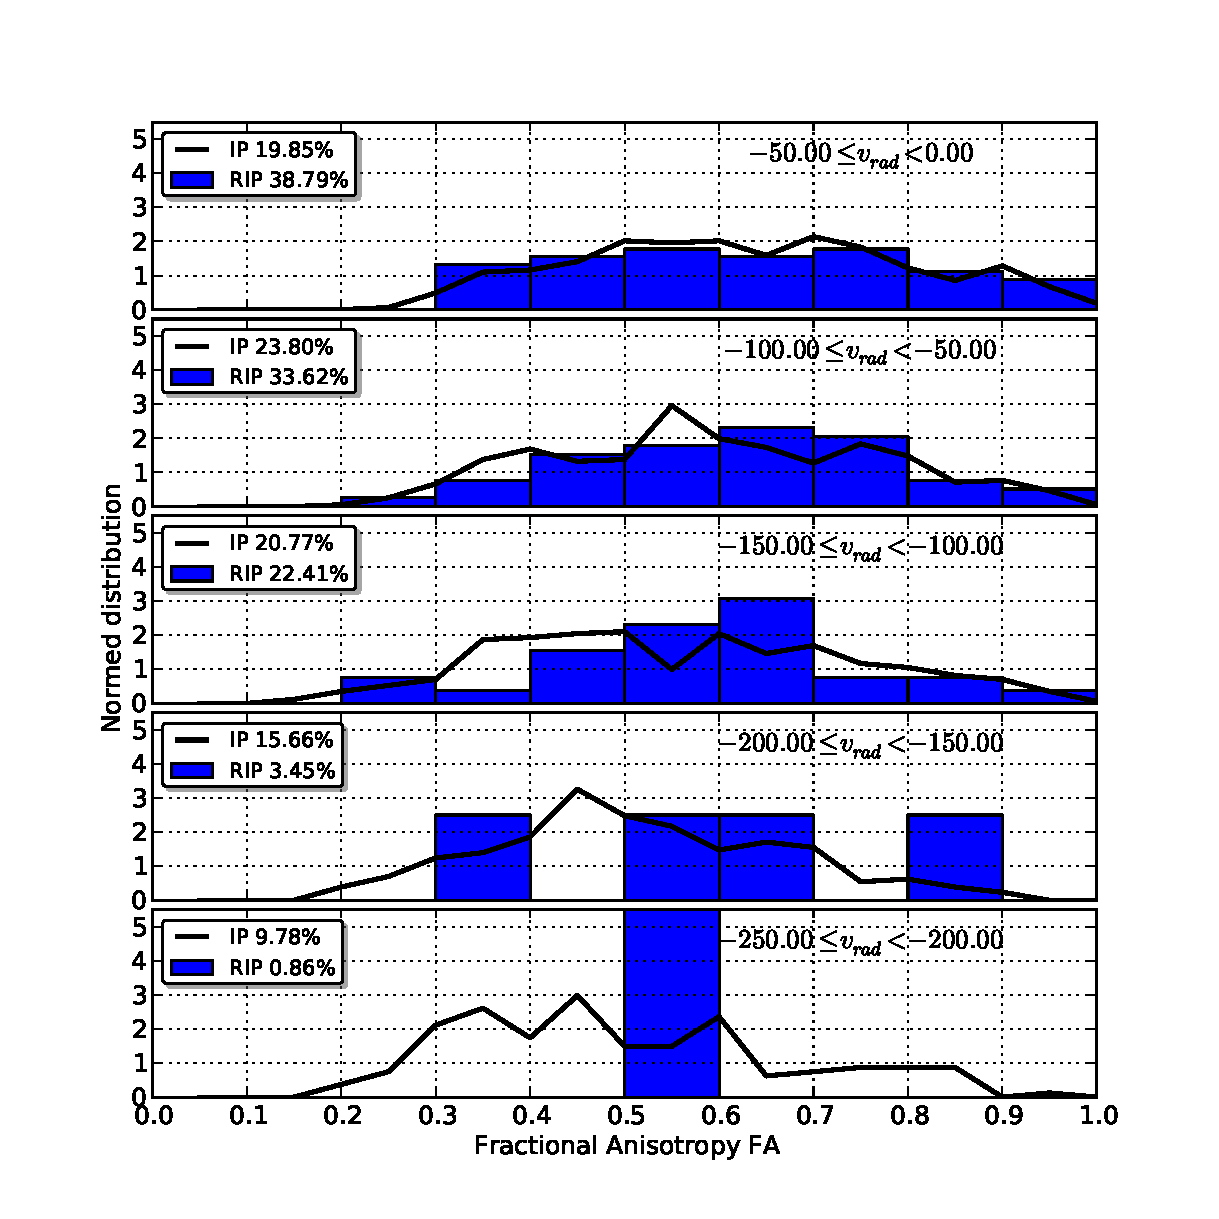
\includegraphics[trim = 4mm 9mm 17mm 15mm, clip, keepaspectratio=true,
  width=0.36\textheight]{./figures/single_radialvelocity_FA_BDM_Tweb}
  
  \captionof{figure}{\small \textit{Left panel:} histograms of the radial 
  velocity of each pair sample, \texttt{IP} (2D histogram) and \texttt{RIP} 
  (blue scatter), vs the fractional anisotropy index associated to each 
  system. In the side panels we compute individual histograms of each one 
  of the analysed properties for \texttt{IP} systems. \textit{Right 
  panel:} selecting different velocity ranges for the radial velocity of 
  the pairs, specified in each single panel, we calculate histograms of 
  the fractional anisotropy of each sample, \texttt{IP} (black lines) and
  \texttt{RIP} (blue bars).}

  \label{fig:radialvelocity_FA}
  \vspace{0.1 cm}

\end{center}
\end{figure*}
\end{flushleft}
%.........................................................................



%.........................................................................
%Distributions of the tangential velocity of pair systems vs the respective 
%FA value
\begin{flushleft}
\begin{figure*}
\begin{center}

  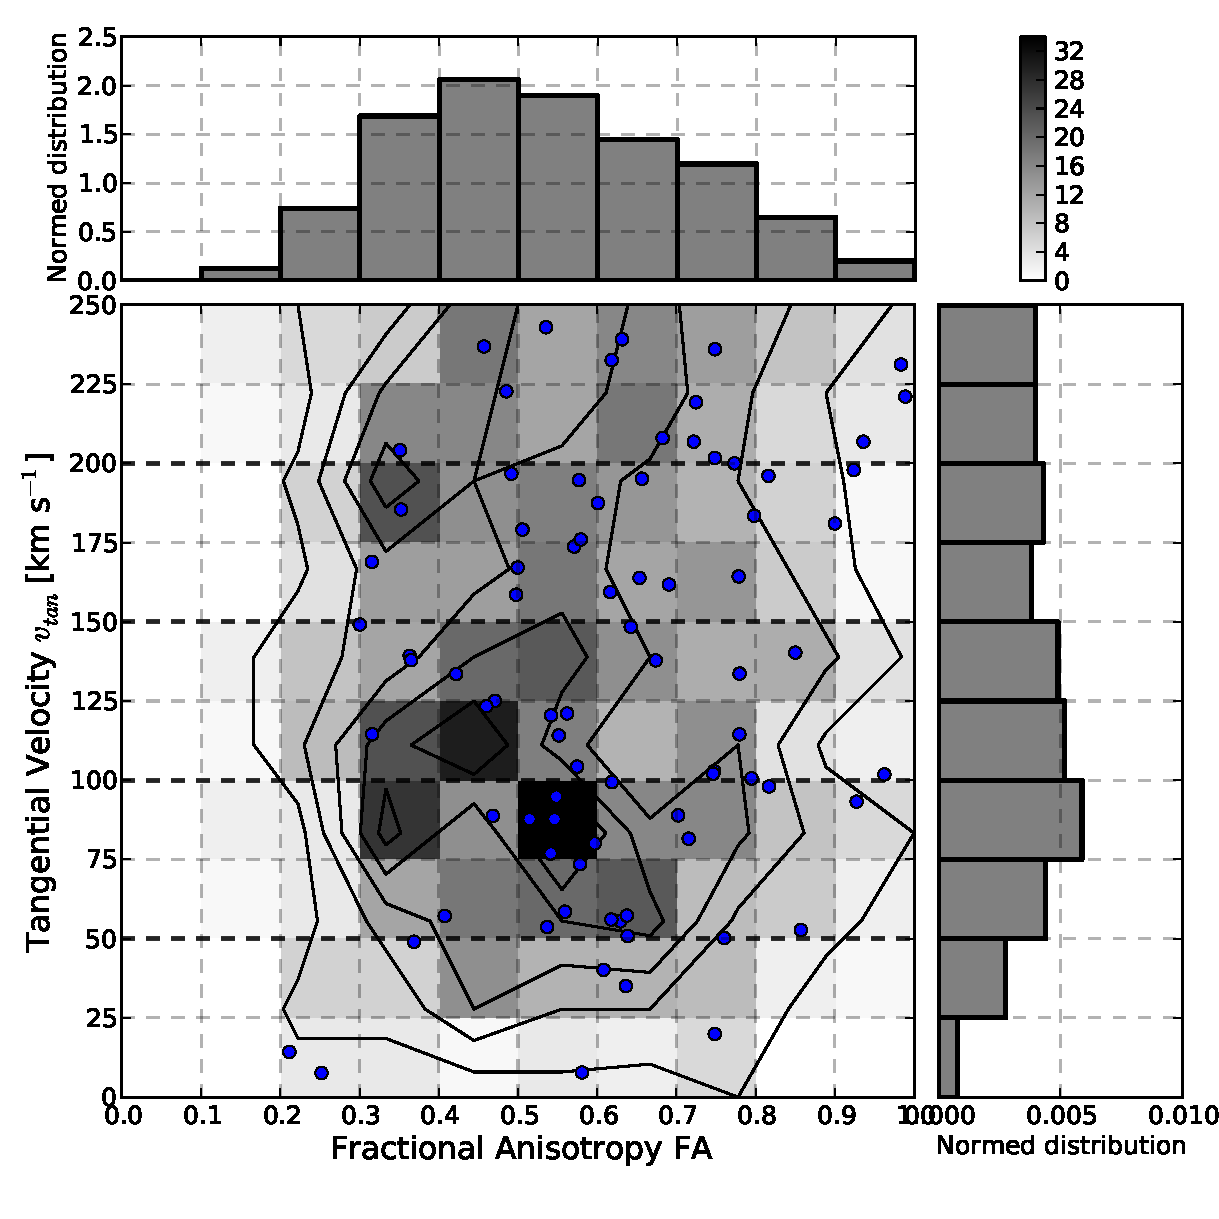
\includegraphics[trim = 2mm 9mm 3mm 4mm, clip, keepaspectratio=true,
  width=0.36\textheight]{./figures/2D_tangentialvelocity_FA_BDM_Tweb}
  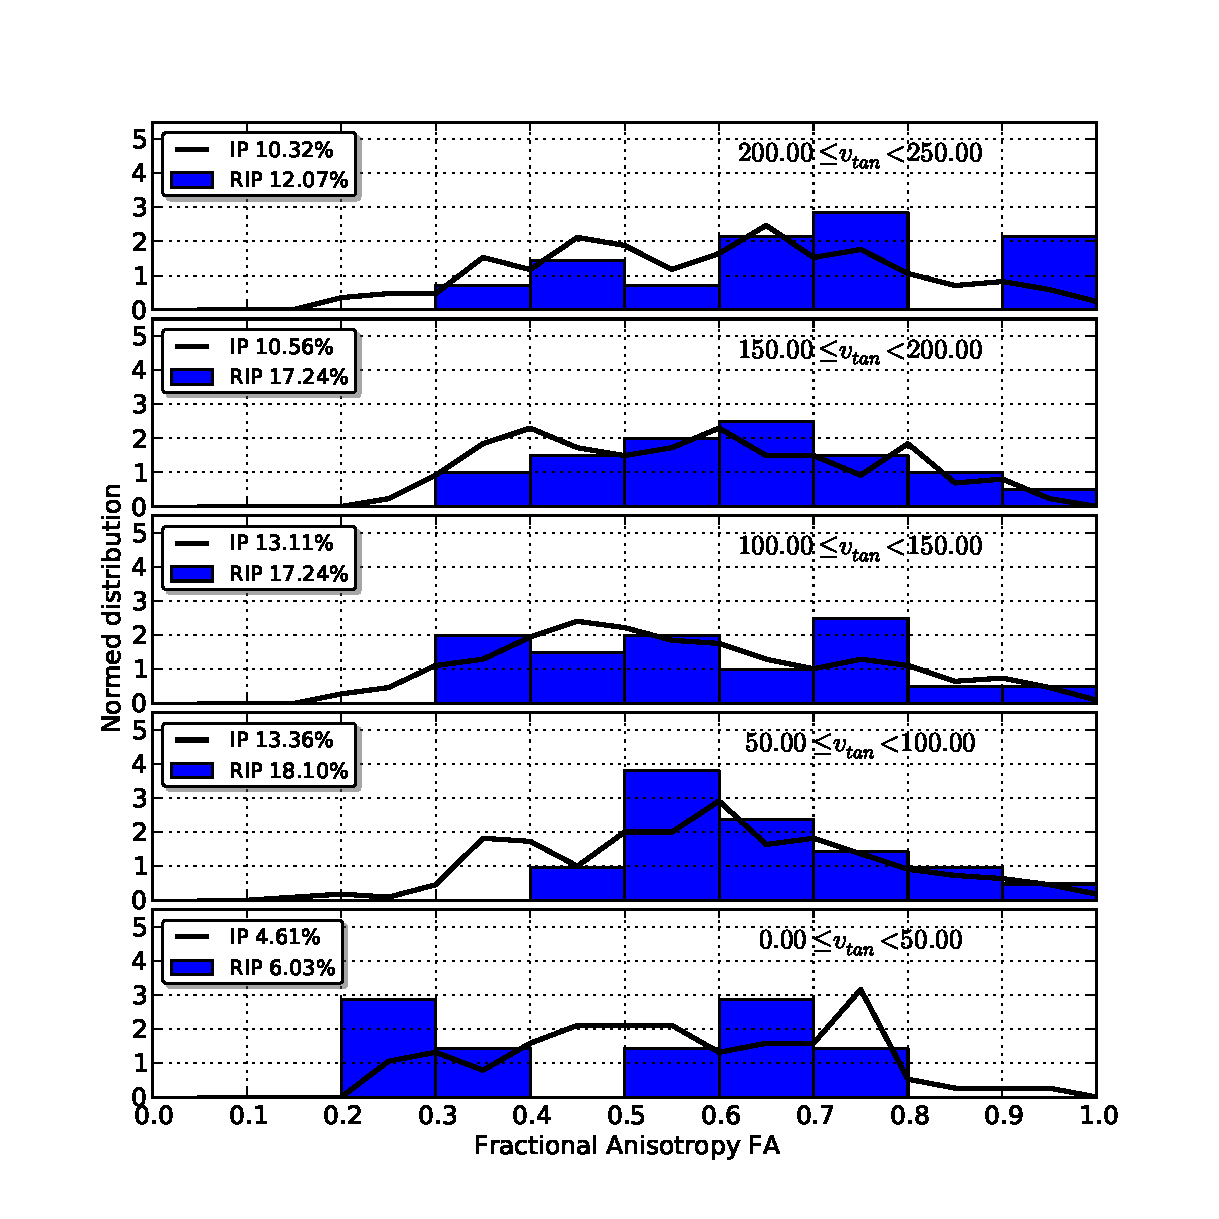
\includegraphics[trim = 4mm 9mm 17mm 15mm, clip, keepaspectratio=true,
  width=0.36\textheight]{./figures/single_tangentialvelocity_FA_BDM_Tweb}
  
  \captionof{figure}{\small \textit{Left panel:} histograms of the 
  tangential velocity of each pair sample, \texttt{IP} (2D histogram) and 
  \texttt{RIP} (blue scatter), vs the fractional anisotropy index 
  associated to each system. In the side panels we compute individual 
  histograms of each one of the analysed properties for \texttt{IP} 
  systems. \textit{Right panel:} selecting different velocity ranges for 
  the radial velocity of the pairs, specified in each single panel, we 
  calculate histograms of the fractional anisotropy of each sample, 
  \texttt{IP} (black lines) and \texttt{RIP} (blue bars).}

  \label{fig:tangentialvelocity_FA}
  \vspace{0.1 cm}

\end{center}
\end{figure*}
\end{flushleft}
%.........................................................................
\end{document}
